\usepackage{etex} %эта магическая херь избавляет от переполнения регистров TeX а!!!

\mode<article>{\usepackage{fullpage}}
\mode<presentation>{
    \usetheme{Madrid}
    \useoutertheme{shadow}
} 

\usepackage[utf8]{inputenc}
\usepackage[russian]{babel}
\usepackage{indentfirst}
\usepackage{graphicx}

\usepackage{amsmath}
\usepackage{amsfonts}
\usepackage{amsthm}
%\usepackage{algorithm}
%\usepackage{algorithmic}

%\usepackage[all]{xy}

\date{Лекция по дисциплине <<методы и средства защиты компьютерной информации>> (\today)}
\author[М.~М.~Шихов]{Михаил Шихов \\ \texttt{\underline{m.m.shihov@gmail.com}}}

%%для рисования графов пакетом xy-pic
%\entrymodifiers={++[o][F-]}

%%для псевдокода алгоритмов (algorithm,algorithmic)
%\renewcommand{\algorithmicrequire}{\textbf{Вход:}}
%\renewcommand{\algorithmicensure}{\textbf{Выход:}}
%\renewcommand{\algorithmiccomment}[1]{// #1}
%\floatname{algorithm}{Псевдокод}

%\setbeamercolor{alerted text}{fg=-green} %gyan, blue, green, -green

\title[Помехоустойчивое кодирование]{Защита целостности. Помехоустойчивое кодирование}


\begin{document}


%титул и содержание статьи
\mode<article>{\maketitle\tableofcontents}

%титул и содержание презентации
\frame<presentation>{\titlepage}
\begin{frame}<presentation>[allowframebreaks]
\frametitle{Содержание}
\tableofcontents
\end{frame}


\section{Передача сообщений}


\subsection{Целостность}


\begin{frame}
    \frametitle{Свойство целостности}
    
    \begin{definition}%theorem, lemma, proof, corollary, example
        \alert{Целостность} информации --- это её неизменность относительно некоторого фиксированного значения.
    \end{definition}
    Например, это свойство дает \alert{получателю} уверенность в том, что он получил информацию в том виде, 
    в котором она была отправлена \alert{источником}. 
    
    В любом канале передачи информации имеется \alert{шум} (источник \alert{помех}), который воздействует 
    на передаваемый \alert{сигнал}, искажая его. 
    
\end{frame}


Рассмотрим схему канала передачи информации, представленную на


\begin{frame}
    \frametitle{Схема канала передачи данных}
    
    \begin{figure}
        \begin{center}
            \mode<presentation>{ 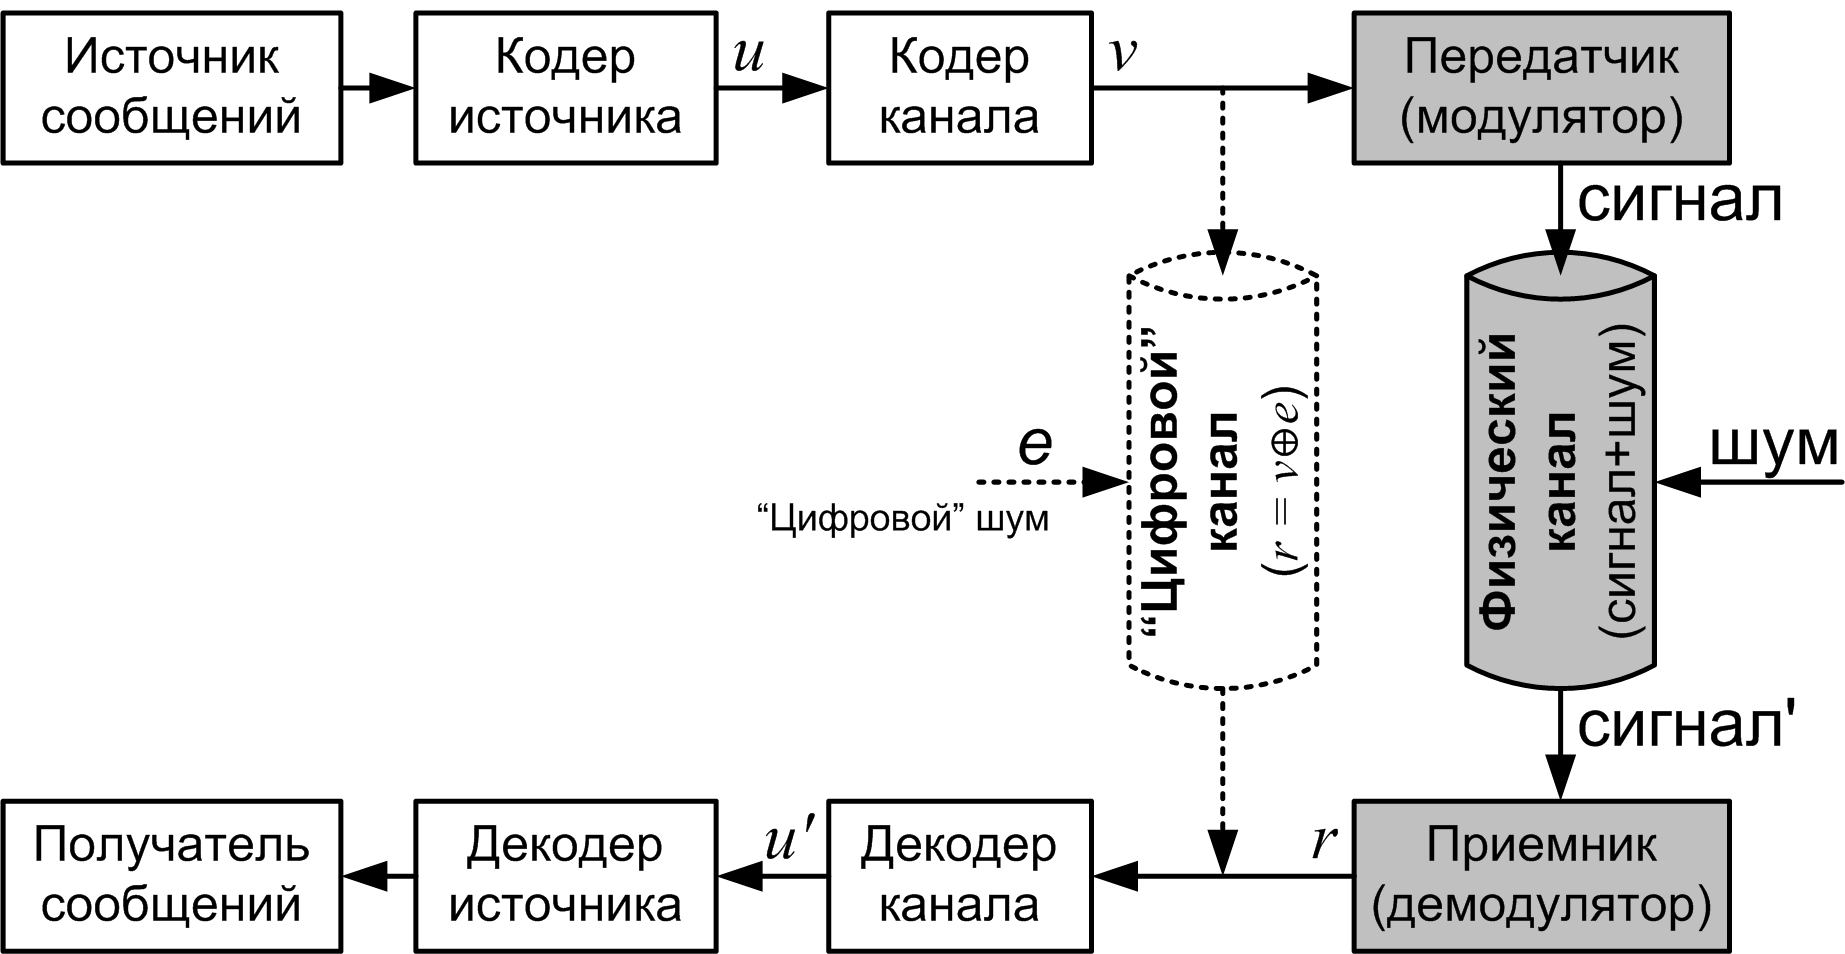
\includegraphics[width=.9\textwidth]{pict/channel} }
            \mode<article>{ 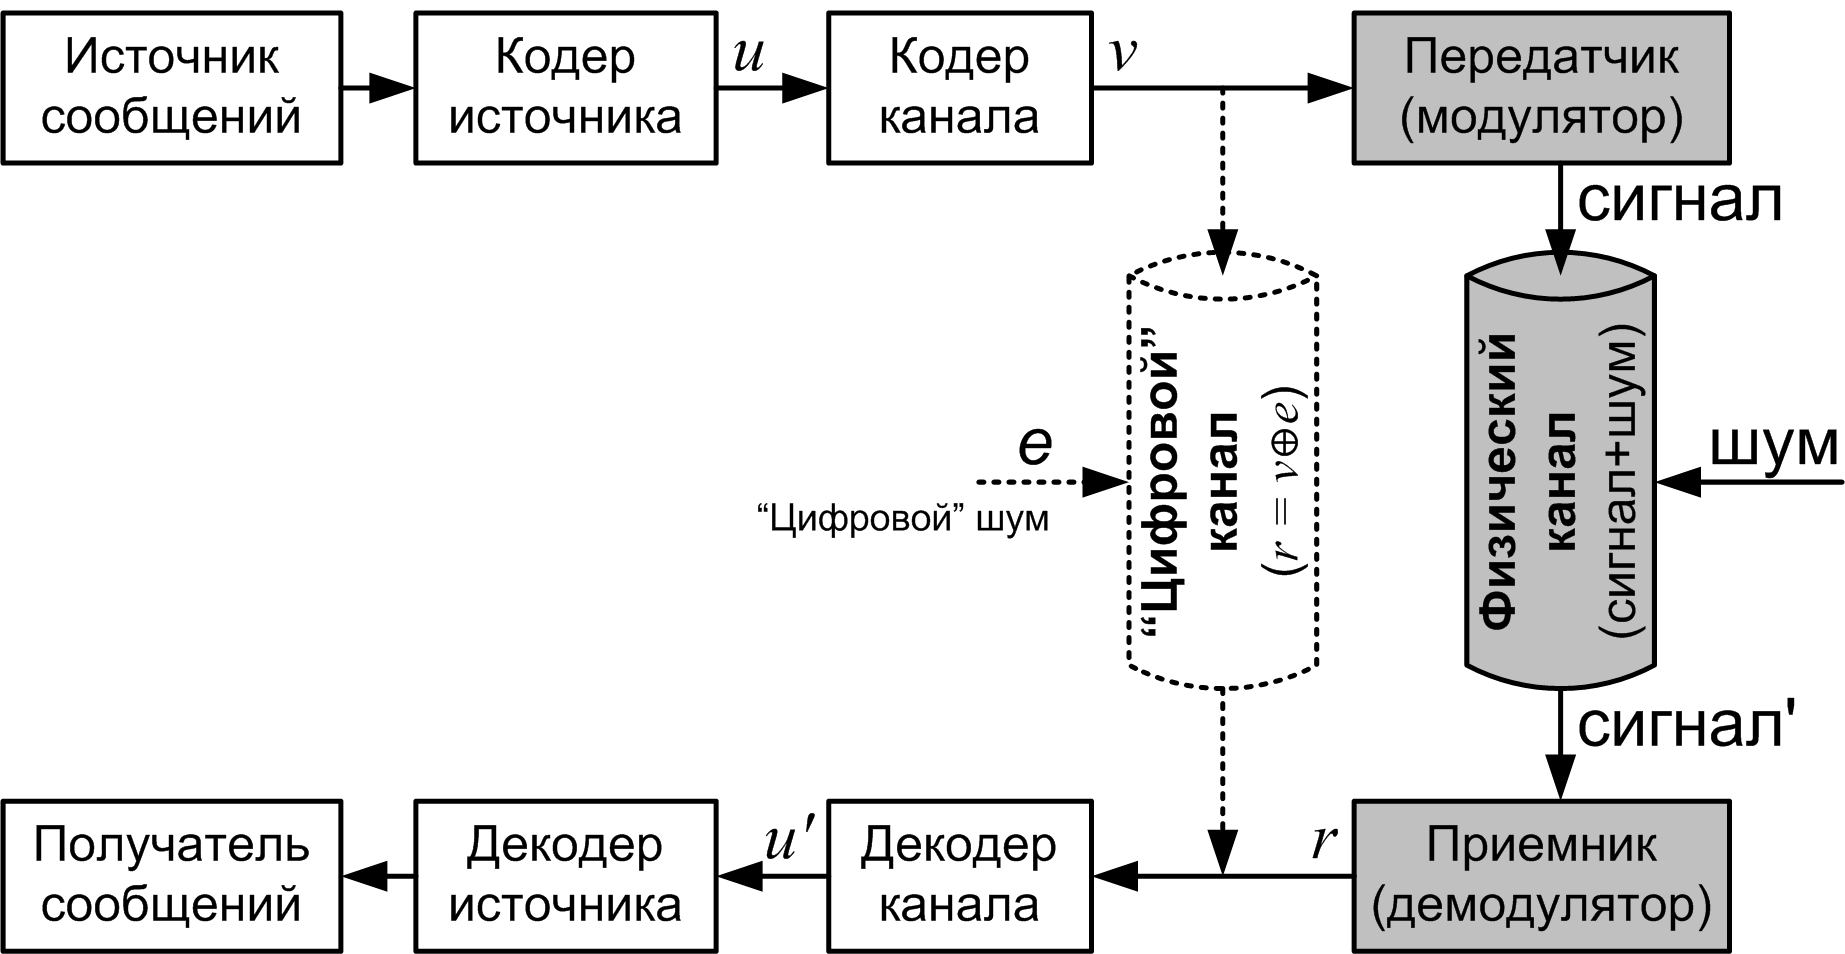
\includegraphics[width=.9\textwidth]{pict/channel} } 
            \caption{Схема канала передачи данных}\label{pict:channel}
        \end{center}
    \end{figure} 
    \mode<article>{См. Рис. \ref{pict:channel}}
\end{frame}


Итак, имеется источник событий (сообщений), которые, поступая на вход \emph{кодера источника}, преобразуются в информацию $u$ (например, в последовательность бит, которую далее называем информационным вектором, или просто вектором). Эта информация адекватно отражает источник и не более того. Далее информационный вектор $u$ поступает на вход \emph{кодера канала}. \emph{Кодер канала}, используя определенные методики перекодирования, добавляет к информации $u$ избыточность, необходимую для защиты от помех и в результате выходе получается вектор $v$. Так как вектор $v$ избыточен, то количество информации в нем больше, чем в $u$. Далее вектор $v$ передается на вход \emph{модулятора}. \emph{Модулятор } преобразует информацию в соответствующий сигнал, распространяющийся в некоторой \emph{физической среде}. Любая \emph{физическая среда} передачи сигнала (физический канал на рисунке) подвержена воздействию шумов (помех). Шум накладывается на сигнал, и результат этого наложения поступает на вход \emph{демодулятора}. Если помехи были несущественными, то на выходе будет вектор $r, r=v$. Иначе, \emph{демодулятор} выдаст вектор $r, r\neq v$. \emph{Декодер канала}, получив на входе вектор $r$, выполнит устранение избыточности, а также постарается распознать были ли в канале ошибки и, возможно, постарается их исправить. На выходе \emph{декодера канала} будет получен вектор $u'$, о котором с большой уверенностью можно сказать, что он идентичен вектору $u$. \emph{Декодер источника} преобразует $u'$ в события (сообщения) удобные для получателя.

\emph{Сигнал} для передачи в физическом канале формируется модулятором из кода $v$, поступившего от \emph{кодера канала}. Совершенствуя модулятор/демодулятор (\emph{модем}), повышая его качество, мы рано или поздно столкнемся с эффектом <<насыщения>>, когда затраты велики, а прирост качества ничтожен. В этом плане совершенствование кодера/декодера (\emph{кодек}) канала дает больший эффект см. Рис. \ref{pict:money2ber}. При этом мы абстрагируемся от того, что у нас вообще есть модем: выход кодека канала $v$ непосредственно <<передается>> в абстрактном <<цифровом>> канале. В этом случае \emph{цифровой аналог шума} --- это информационный вектор $e$, накладывающийся по xor на вектор $v$.

Совершенствованием \emph{кодека} мы и займемся. <<Качество>> цифрового канала оценивается средней долей ошибочных бит (BER --- Bit Error Rate). BER определяется как средняя вероятность ошибки одного бита передаваемой информации. Чем BER меньше, тем лучше, на рисунке же Рис. \ref{pict:money2ber} под <<качеством>> понималась величина обратная к BER, например, 1/BER.

\begin{frame}
    \frametitle{Зависимость качества от затрат}
    
    \begin{definition}
        BER (Bit Error Rate) --- средняя доля ошибочных бит (вероятность ошибки (инвертирования) при передаче одного бита информации).
    \end{definition}
    
    \begin{figure}
        \begin{center}
            \mode<presentation>{ 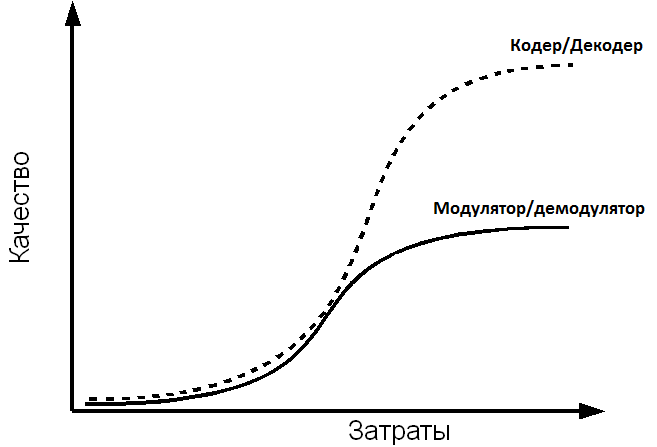
\includegraphics[height=.5\textheight]{pict/money2ber} }
            \mode<article>{ 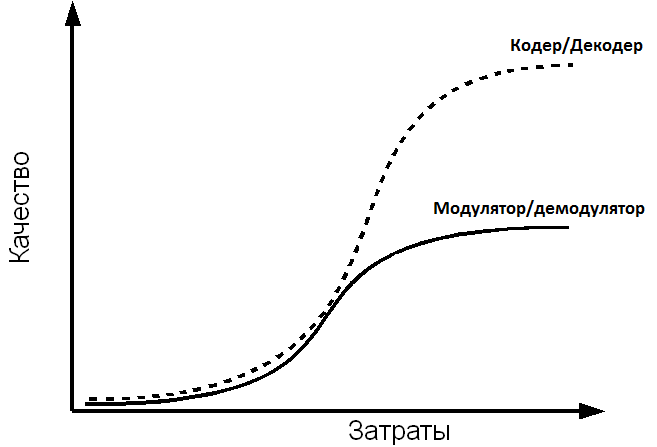
\includegraphics[width=.9\textwidth]{pict/money2ber} } 
            \caption{Зависимость качества от затрат}\label{pict:money2ber}
        \end{center}
    \end{figure} 
    \mode<article>{См. Рис. \ref{pict:money2ber}}
    
\end{frame}


\begin{frame}
    \frametitle{Типы ошибок в <<цифровом>> канале}
    
    \begin{itemize}
        \item \alert{Замещение} символа\footnote{Цифры, кодового символа} (в случае двоичного кодирования --- инверсия двоичного разряда).
        
        \item Вставка символа (например, добавление бита в сообщение).
        
        \item Выпадение символа (например, исключение бита из сообщения).
    \end{itemize} 
    Далее будем рассматривать только ошибки \alert{замещения}.
\end{frame}


\begin{frame}
    \frametitle{Принципы и стратегии помехоустойчивого кодирования}
    
    Необходимо внести в исходное кодовое слово $u$ дополнительные служебные биты информации, предназначенные для повышения устойчивости к помехам. В результате исходное кодовое слово $u$ будет преобразовано кодером канала в слово $v$ большей длины.
    
    Существуют две стратегии борьбы с помехами:
    \begin{itemize}
        \item с обнаружением ошибок и с последующим запросом на повторную передачу (ARQ --- Automatic Repeat Request).
    
        \item с непосредственным обнаружением и исправлением ошибок на стороне получателя (FEC --- Forvard Error Correction);        
    \end{itemize}
\end{frame}


\section{Стратегии}


\subsection{ARQ}


Рассмотрим ARQ стратегию на примере ИНН --- идентификационного номера налогоплательщика. С этими номерами работают люди и ошибки неизбежны. Что будет, если оператор допустит ошибку при вводе такого кода? Ничего хорошего. Поэтому в ИНН есть цифры контрольного кода. Формат ИНН(различают ИНН для юридических лиц (ЮЛ) и для физических лиц (ФЛ)) представлен на рисунке Рис. \ref{pict:inn}. 

\begin{frame}
    \frametitle{ARQ}
    \framesubtitle{Структура ИНН}
    
    \begin{figure}
        \begin{center}
            \mode<presentation>{ 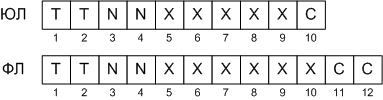
\includegraphics[width=.6\textwidth]{pict/inn} }
            \mode<article>{ 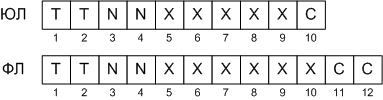
\includegraphics[width=.6\textwidth]{pict/inn} } 
            \caption{Структура ИНН}\label{pict:inn}
        \end{center}
    \end{figure}
    \mode<article>{См. Рис. \ref{pict:inn}}
    \alert{TT} --- код территориального деления (номер региона), \alert{NN} --- номер инспекции в регионе, \alert{X} --- порядковый номер налогоплательщика в инспекции, \alert{C} --- контрольный код.
\end{frame}


\begin{frame}
    \frametitle{Веса разрядов ИНН}
    \begin{table}[ht]
        \caption{Веса разрядов ИНН}\label{t:innWeights}
        \centering
        \begin{tabular}[c]{|l|l|l|l|}
            \hline\hline
            Номер разряда $i$   &$a_i$  &$b_i$  &$c_i$ \\
            \hline
            1                   &2      &7      &3 \\
            2                   &4      &2      &7 \\
            3                   &10     &4      &2 \\
            4                   &3      &10     &4 \\
            5                   &5      &3      &10\\
            6                   &9      &5      &3 \\
            7                   &4      &9      &5 \\
            8                   &6      &4      &9 \\
            9                   &8      &6      &4 \\
            10                  &       &8      &6 \\
            11                  &       &       &8 \\
            \hline
        \end{tabular}
    \end{table}
    \mode<article>{См. Табл. \ref{t:innWeights}}
\end{frame}


\begin{frame}
    \frametitle{ARQ}
    \framesubtitle{Структура ИНН}
    
    Расчет контрольных цифр для ИНН юридического лица производится так:
    \[ \text{ЮЛ}_{10}=\left(\left(\sum_{i=1}^9\text{ЮЛ}_i\cdot a_i\right)\bmod 11\right)\bmod 10. \]
    
    Для физического лица:
    \[ \text{ФЛ}_{11}=\left(\left(\sum_{i=1}^{10}\text{ФЛ}_i\cdot b_i\right)\bmod 11\right)\bmod 10. \]
    \[ \text{ФЛ}_{12}=\left(\left(\sum_{i=1}^{11}\text{ФЛ}_i\cdot c_i\right)\bmod 11\right)\bmod 10. \]
    
\end{frame}


\begin{frame}
    \frametitle{ARQ}
    \framesubtitle{Структура ИНН}

    \begin{example}[Контрольный код]
        Есть физическое лицо, закрепленное под номером 832630 в налоговой инспекции номер 45 в Кировской области. Сформировать корректный контрольный код для его ИНН=4345832630\fbox{\alert{??}}. 
    \end{example}
    
    \[
    \begin{split}
        \text{ФЛ}_{11}=
        \left(
            \left(
                \begin{split}
                    4\cdot 7+3\cdot 2+4\cdot 4+5\cdot 10+8\cdot 3+\\
                    +3\cdot 5+2\cdot 9+6\cdot 4+3\cdot 6+0\cdot 8
                \end{split}
            \right)\bmod 11
        \right)\bmod 10=\\
        =(199 \bmod 11)\bmod 10=1 \bmod 10=\fbox{1},
        \text{ФЛ}_{12}=\\=
        \left(
            \left(
                \begin{split}
                    4\cdot 3+3\cdot 7+4\cdot 2+5\cdot 4+8\cdot 10+\\
                    +3\cdot 3+2\cdot 5+6\cdot 9+3\cdot 4+0\cdot 6+1\cdot 8
                \end{split}
            \right)\bmod 11
        \right)\bmod 10=\\
        =(234 \bmod 11)\bmod 10=3 \bmod 10=\fbox{3}.
    \end{split}    
    \]
\end{frame}


Получаем ИНН=4345832630\fbox{\alert{13}}.


\begin{frame}
    \frametitle{ARQ}
    \framesubtitle{Структура ИНН}

    \begin{example}[Неверный ввод]
        ИНН=4345832630\fbox{\alert{13}}. Допустим, оператор вводил данный ИНН и ошибся, введя ИНН=434\fbox{6}83263013.
    \end{example}
    \[
    \begin{split}
        \text{ФЛ}_{11}=
        \left(
            \left(
                \begin{split}
                    4\cdot 7+3\cdot 2+4\cdot 4+\fbox{6}\cdot 10+8\cdot 3+\\
                    +3\cdot 5+2\cdot 9+6\cdot 4+3\cdot 6+0\cdot 8
                \end{split}
            \right)\bmod 11
        \right)\bmod 10=\\
        =(209 \bmod 11)\bmod 10=0 \bmod 10=\fbox{0},
        \text{ФЛ}_{12}=\\=
        \left(
            \left(
                \begin{split}
                    4\cdot 3+3\cdot 7+4\cdot 2+\fbox{6}\cdot 4+8\cdot 10+\\
                    +3\cdot 3+2\cdot 5+6\cdot 9+3\cdot 4+0\cdot 6+0\cdot 8
                \end{split}
            \right)\bmod 11
        \right)\bmod 10=\\
        =(230 \bmod 11)\bmod 10=10 \bmod 10=\fbox{0}.
    \end{split}    
    \]
\end{frame}

Введенный контрольный код 13 и рассчитанный 00 не совпали, и система выдала оператору сообщение с просьбой перепроверить введенный ИНН.

\begin{frame}
    \frametitle{ARQ}
    \framesubtitle{Другие примеры}

    \begin{itemize}
        \item Контроль по четности (нечетности) слова $d_{n-1}\cdots d_0$.
        \[ d_{n-1}\cdots d_0 p_\text{четн}, p_\text{четн}=d_{n-1}\oplus\ldots\oplus d_0; \]
        \[ d_{n-1}\cdots d_0 p_\text{нечетн}, p_\text{нечетн}=d_{n-1}\oplus\ldots\oplus d_0\oplus 1. \]
        
        \item Контроль по хеш-функции (контрольной сумме) сообщения $M$.
        \[ M\to \langle M,H(M) \rangle \]
    \end{itemize}
\end{frame}


\subsection{FEC}


Перейдем к стратегии FEC. Ошибки выявляются и исправляются на принимающей стороне. Основная идея, лежащая в такой стратегии заключена в общих словах в том, что каждому исходному кодовому слову\footnote{То есть обычно предполагается, что длина кодового слова фиксирована (а стало быть известно и количество слов кодовых слов)} $u_i$ после обработки кодером канала, соответствует код $v_i$ с внесенной избыточностью. Необходимо отметить, что общее количество всех возможных кодов $v$ значительно больше, чем количество всех возможных кодов $u$. 

Когда в коде $v_i$, вследствие воздействия шума $e$ инвертируется один или несколько бит, он перейдет в код $r_i$. Все возможные коды $r$ отображаются на коды $u'$ (при этом, очевидно одному коду $u'$ соответствует несколько кодов $r$). 


\begin{frame}
    \frametitle{FEC}
    \framesubtitle{Ошибка обнаружена и верно исправлена}
    
    \begin{figure}
        \begin{center}
            \mode<presentation>{ 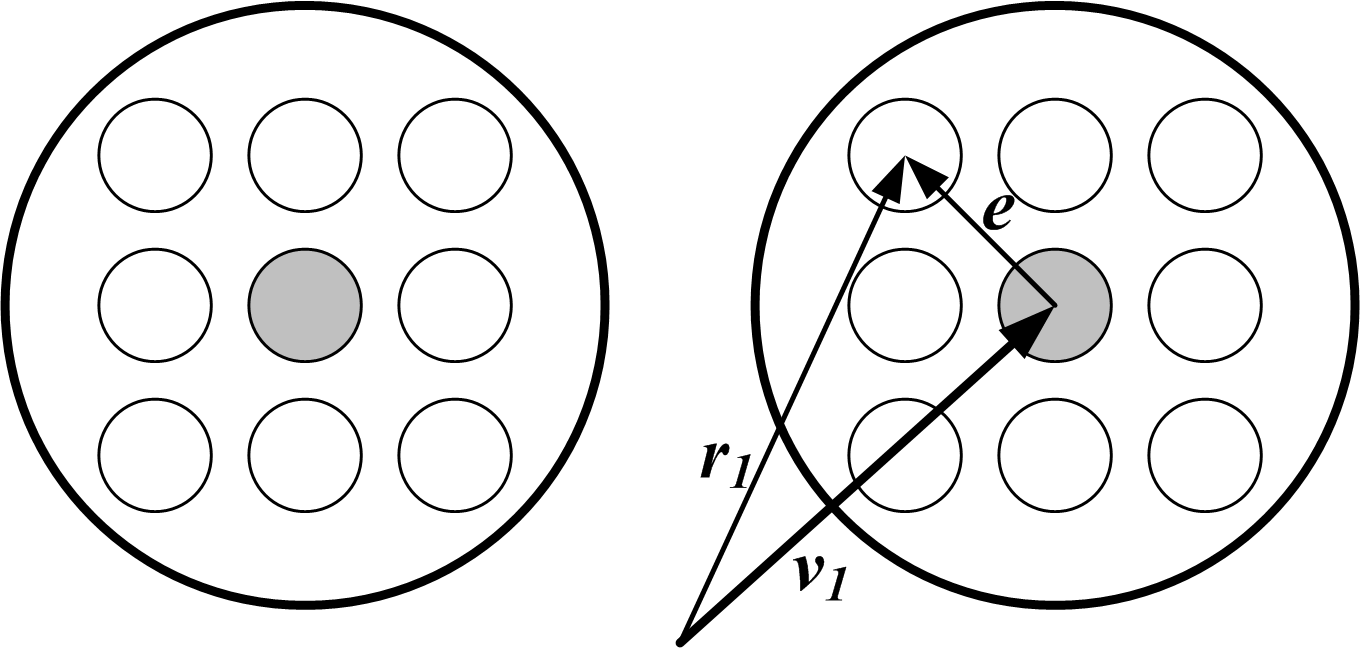
\includegraphics[width=.8\textwidth]{pict/fecOk} }
            \mode<article>{ 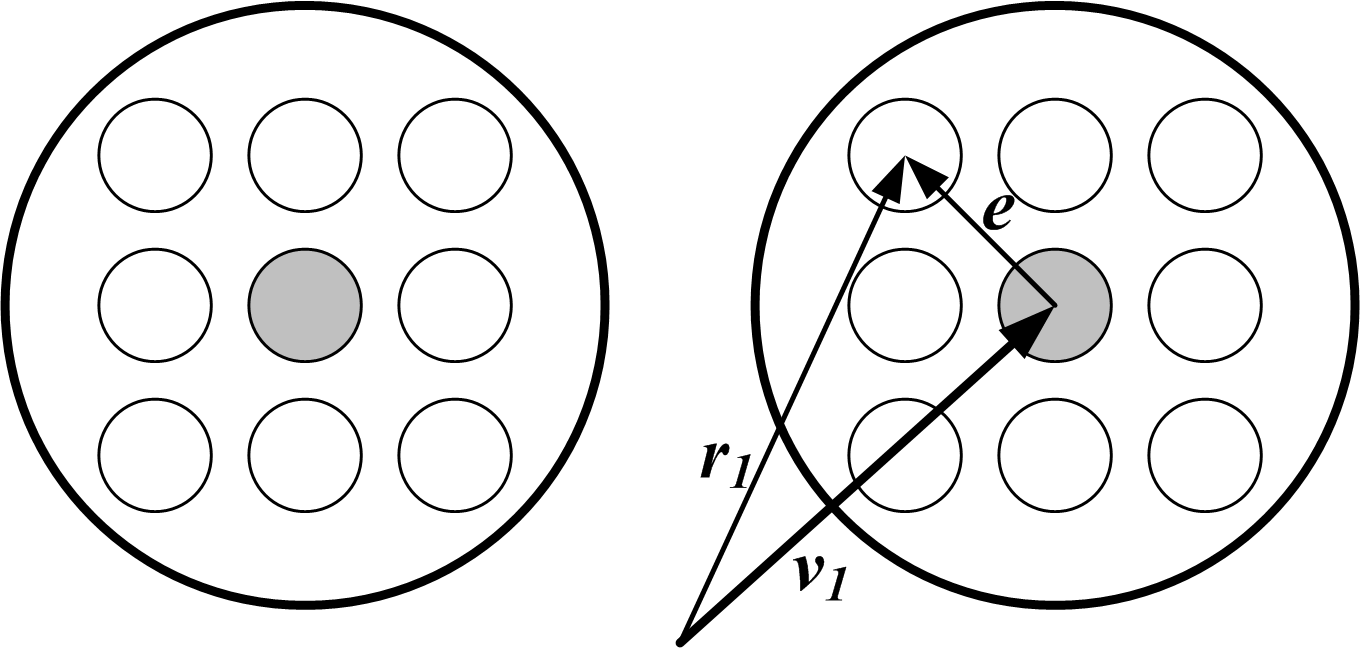
\includegraphics[width=.7\textwidth]{pict/fecOk} } 
            \caption{Ошибка исправлена}\label{pict:fecOk}
        \end{center}
    \end{figure} 
    \mode<article>{См. Рис. \ref{pict:fecOk}}
\end{frame}


\begin{frame}
    \frametitle{FEC}
    \framesubtitle{Ошибка обнаружена, но исправлена неверно}
    
    \begin{figure}
        \begin{center}
            \mode<presentation>{ 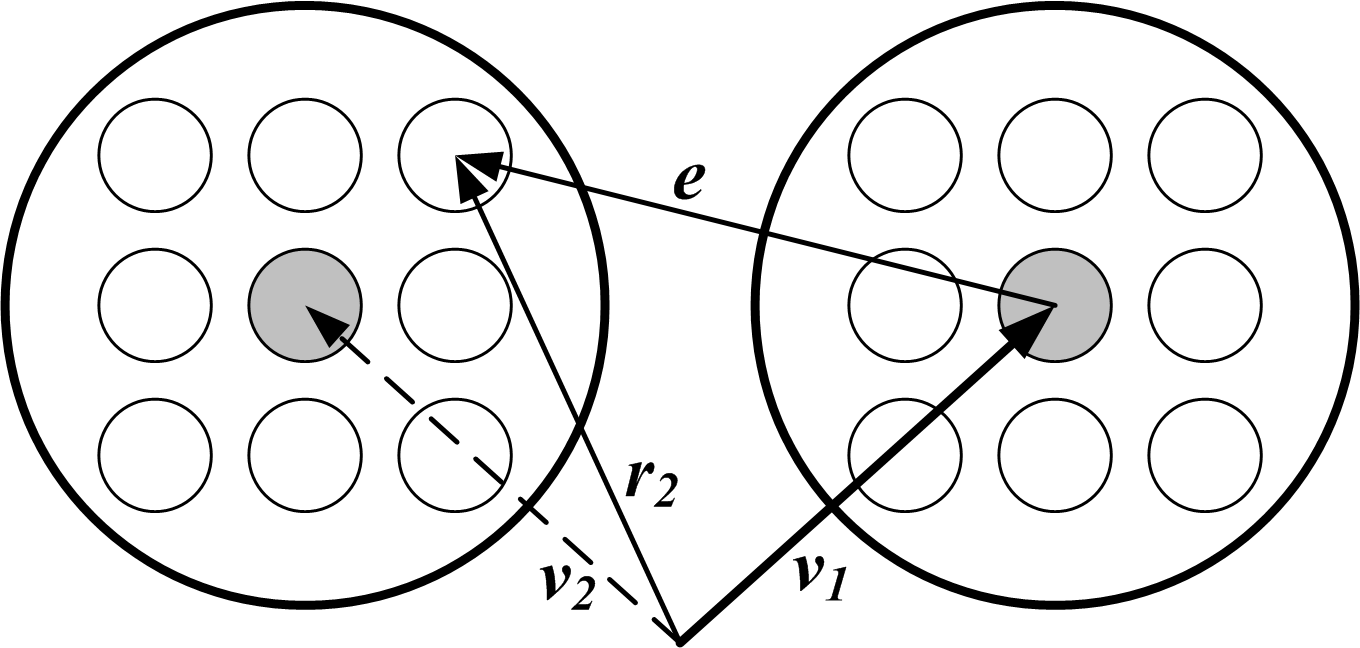
\includegraphics[width=.8\textwidth]{pict/fecIncorrect} }
            \mode<article>{ 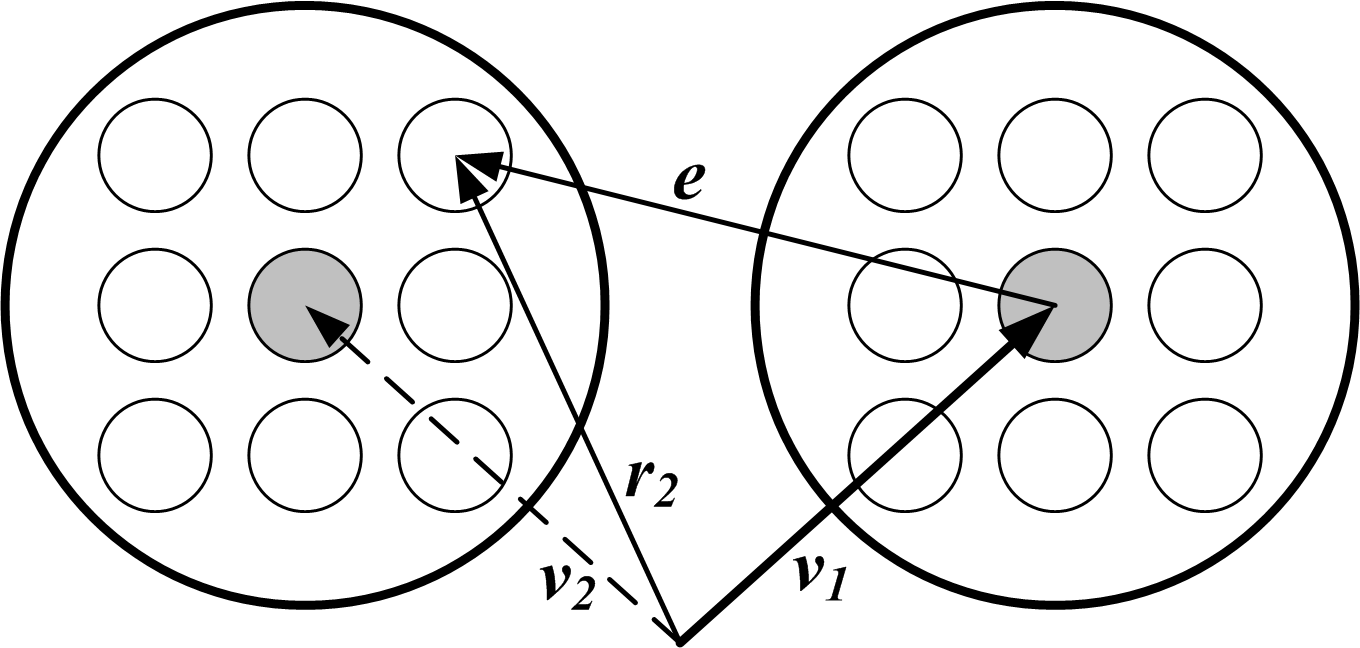
\includegraphics[width=.7\textwidth]{pict/fecIncorrect} } 
            \caption{Ошибка исправлена неверно}\label{pict:fecIncorrect}
        \end{center}
    \end{figure} 
    \mode<article>{См. Рис. \ref{pict:fecIncorrect}}
\end{frame}


\begin{frame}
    \frametitle{FEC}
    \framesubtitle{Необнаружимая ошибка}
    
    \begin{figure}
        \begin{center}
            \mode<presentation>{ 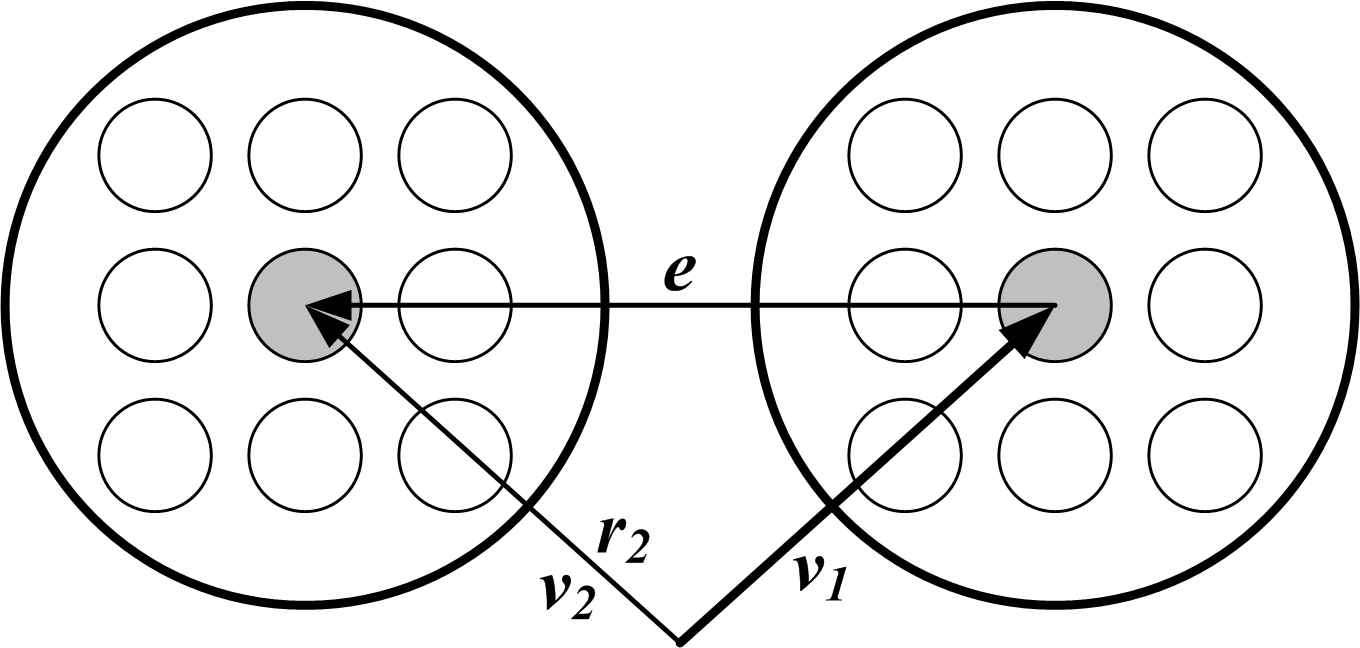
\includegraphics[width=.8\textwidth]{pict/fecFail} }
            \mode<article>{ 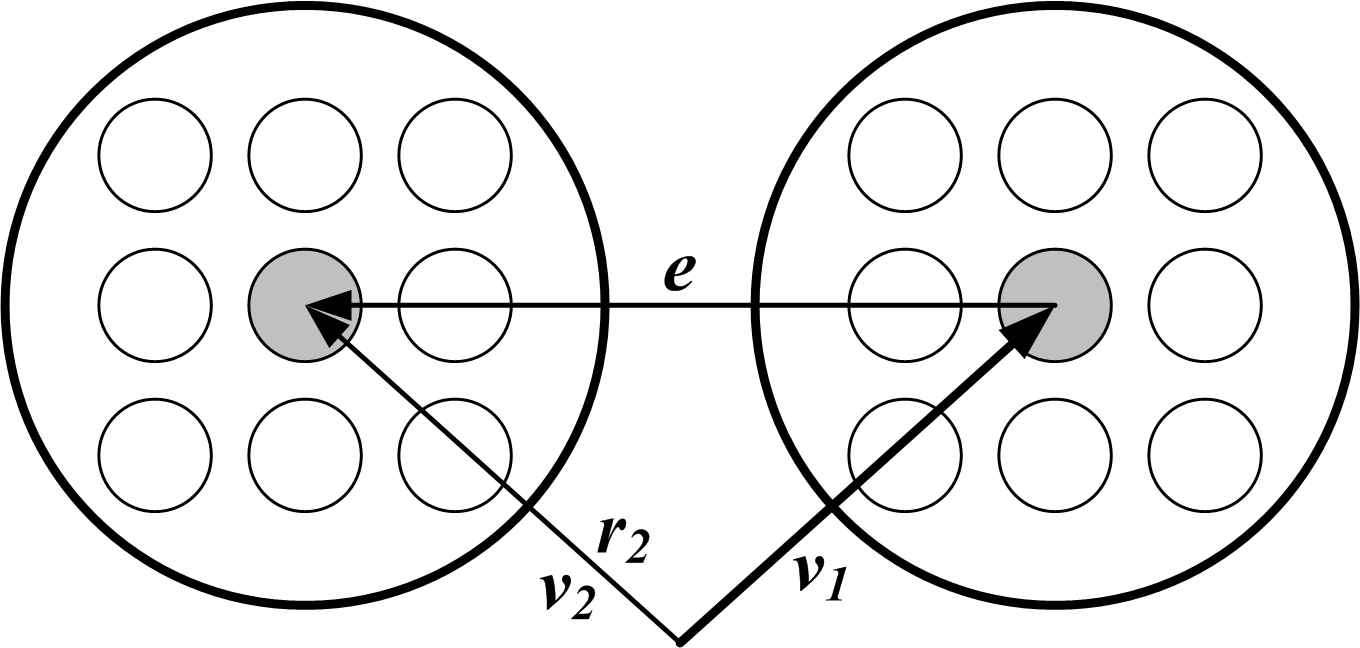
\includegraphics[width=.7\textwidth]{pict/fecFail} } 
            \caption{Ошибка не может быть обнаружена}\label{pict:fecFail}
        \end{center}
    \end{figure} 
    \mode<article>{См. Рис. \ref{pict:fecFail}}
\end{frame}


Подавляющее число ошибок в современных каналах являются одиночными, так как современные каналы имеют достаточно низкий показатель BER. Например, для волоконно-оптических каналов BER равен приблизительно $10^{-12}$. Рассмотрим несколько примеров кодирования для исправления одиночной ошибки.


\begin{frame}
    \frametitle{FEC}
    \framesubtitle{Пример помехоустойчивого кодирования <<утроением>>}

    \begin{itemize}
        \item Схема кодирования $u\to v$.
        \[
            \langle
                0\to 000,1\to 111
            \rangle
        \]
        
        \item Схема декодирования $r\to u'$.
        \[
            \left\langle
                \begin{split}
                    000\to 0,001\to 0,010\to 0,100\to 0,\\
                    111\to 1,110\to 1,101\to 1,011\to 1
                \end{split}
            \right\rangle
        \]
    \end{itemize}
    
    \begin{example}
    Передаётся слово: 101. Кодируется: 111000111. Поступает в канал. Возникает ошибка: 11\fbox{0}000111. Декодируется: 101. При этом декодер <<обнаруживает и верно исправляет>> возникшую ошибку.
    \end{example}
\end{frame}


\begin{frame}
    \frametitle{FEC}
    \framesubtitle{Пример помехоустойчивого кодирования <<утроением>>}
    
    \begin{figure}
        \begin{center}
            \mode<presentation>{ 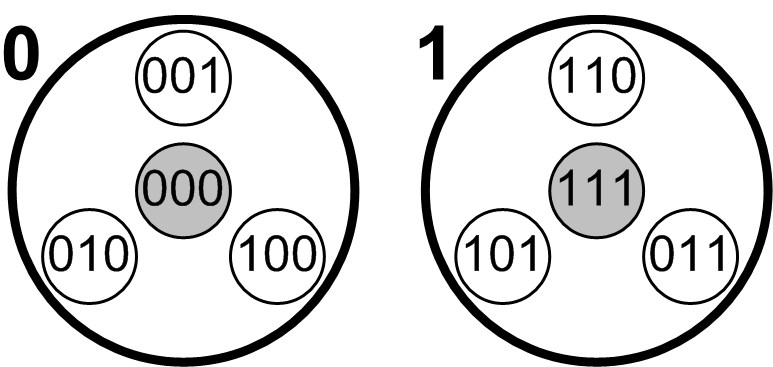
\includegraphics[width=.8\textwidth]{pict/fecTriplet} }
            \mode<article>{ 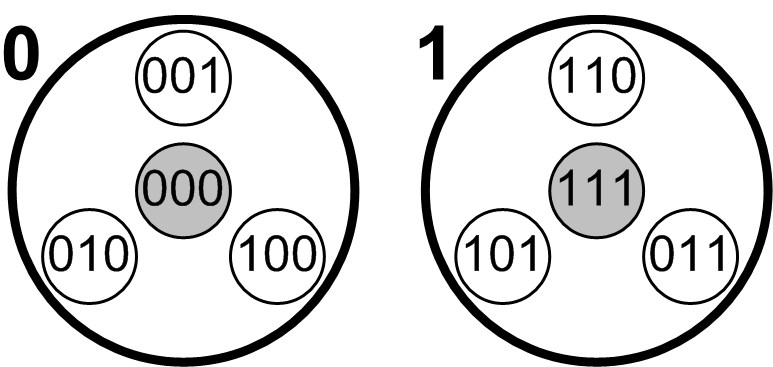
\includegraphics[width=.7\textwidth]{pict/fecTriplet} } 
            \caption{Кластеры при кодировании <<утроением>>}\label{pict:fecTriplet}
        \end{center}
    \end{figure} 
    \mode<article>{См. Рис. \ref{pict:fecTriplet}}
\end{frame}


Конечно, приведенный код слишком избыточен, он увеличивает нагрузку на канал передачи данных в три раза. Это недопустимо. Нужны более экономичные методы. Метод, дающий некоторую ощутимую экономию, приведен на рисунке Рис. \ref{pict:matrix}. Исходное слово укладывается построчно в матрицу. И для каждого столбца и строки формируются избыточные биты контроля по четности.


\begin{frame}
    \frametitle{FEC}
    \framesubtitle{Матричный контроль по четности}
    
    \begin{figure}
        \begin{center}
            \mode<presentation>{ 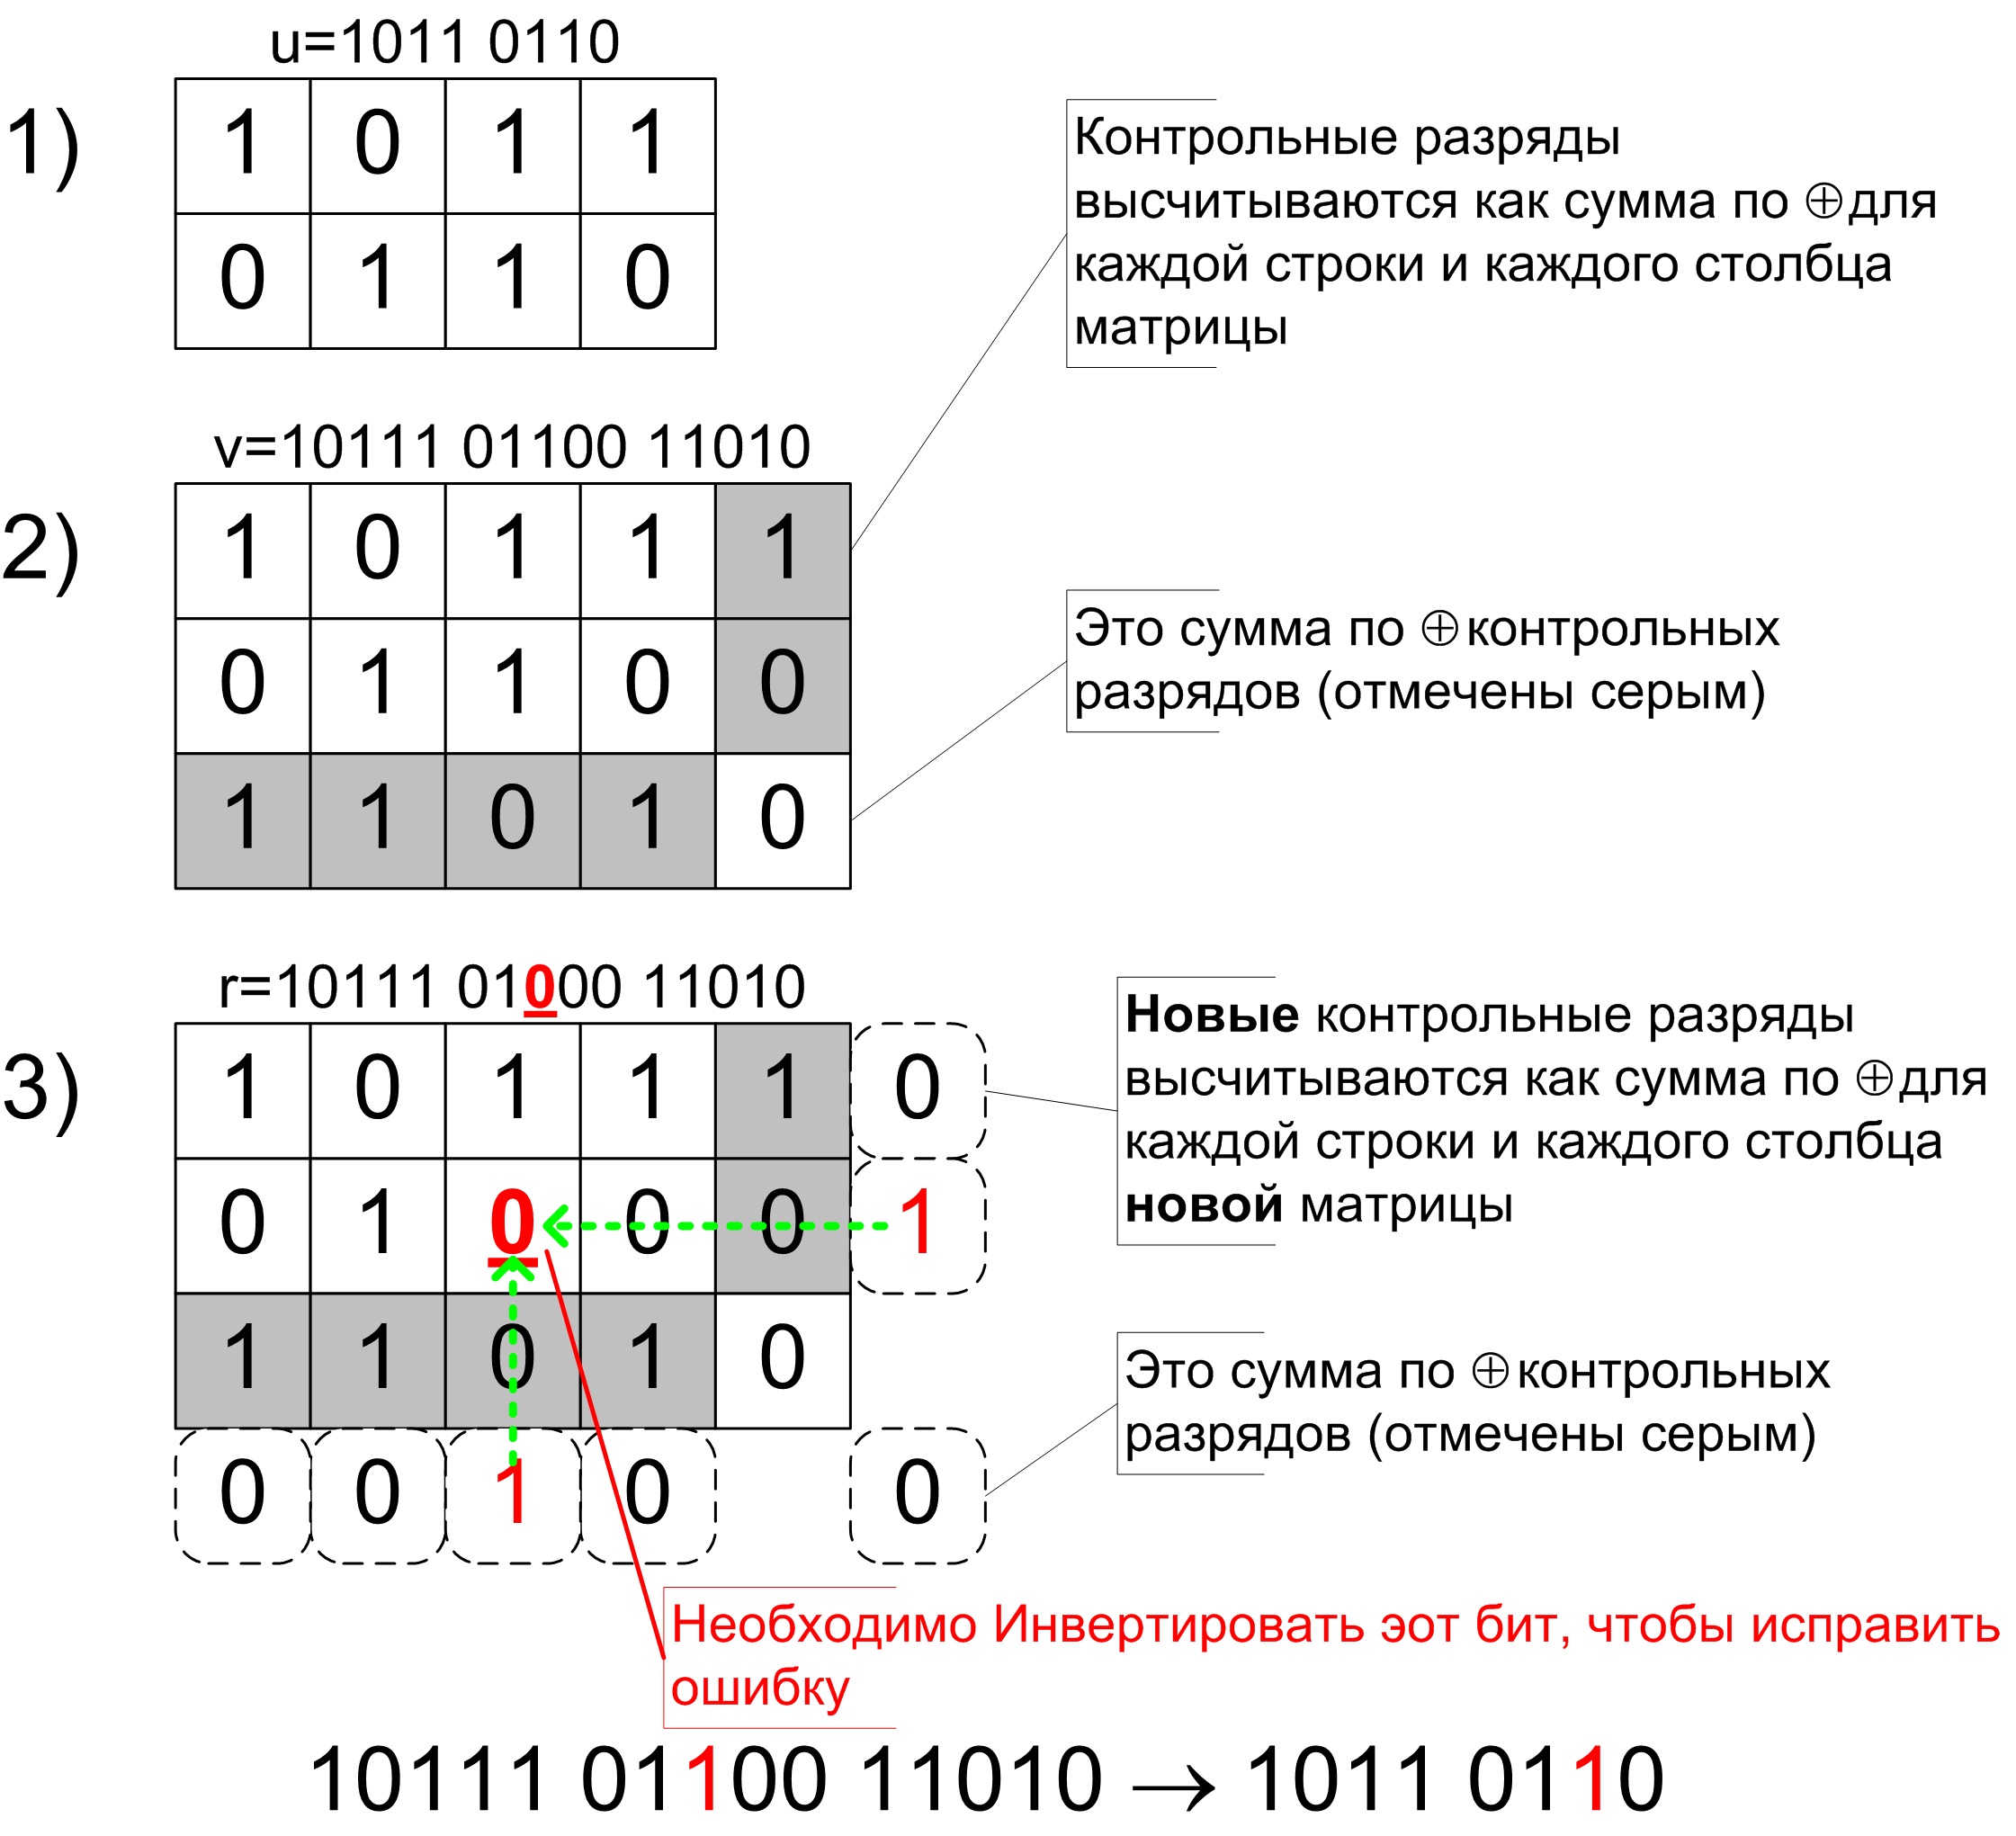
\includegraphics[height=.72\textheight]{pict/matrix} }
            \mode<article>{ 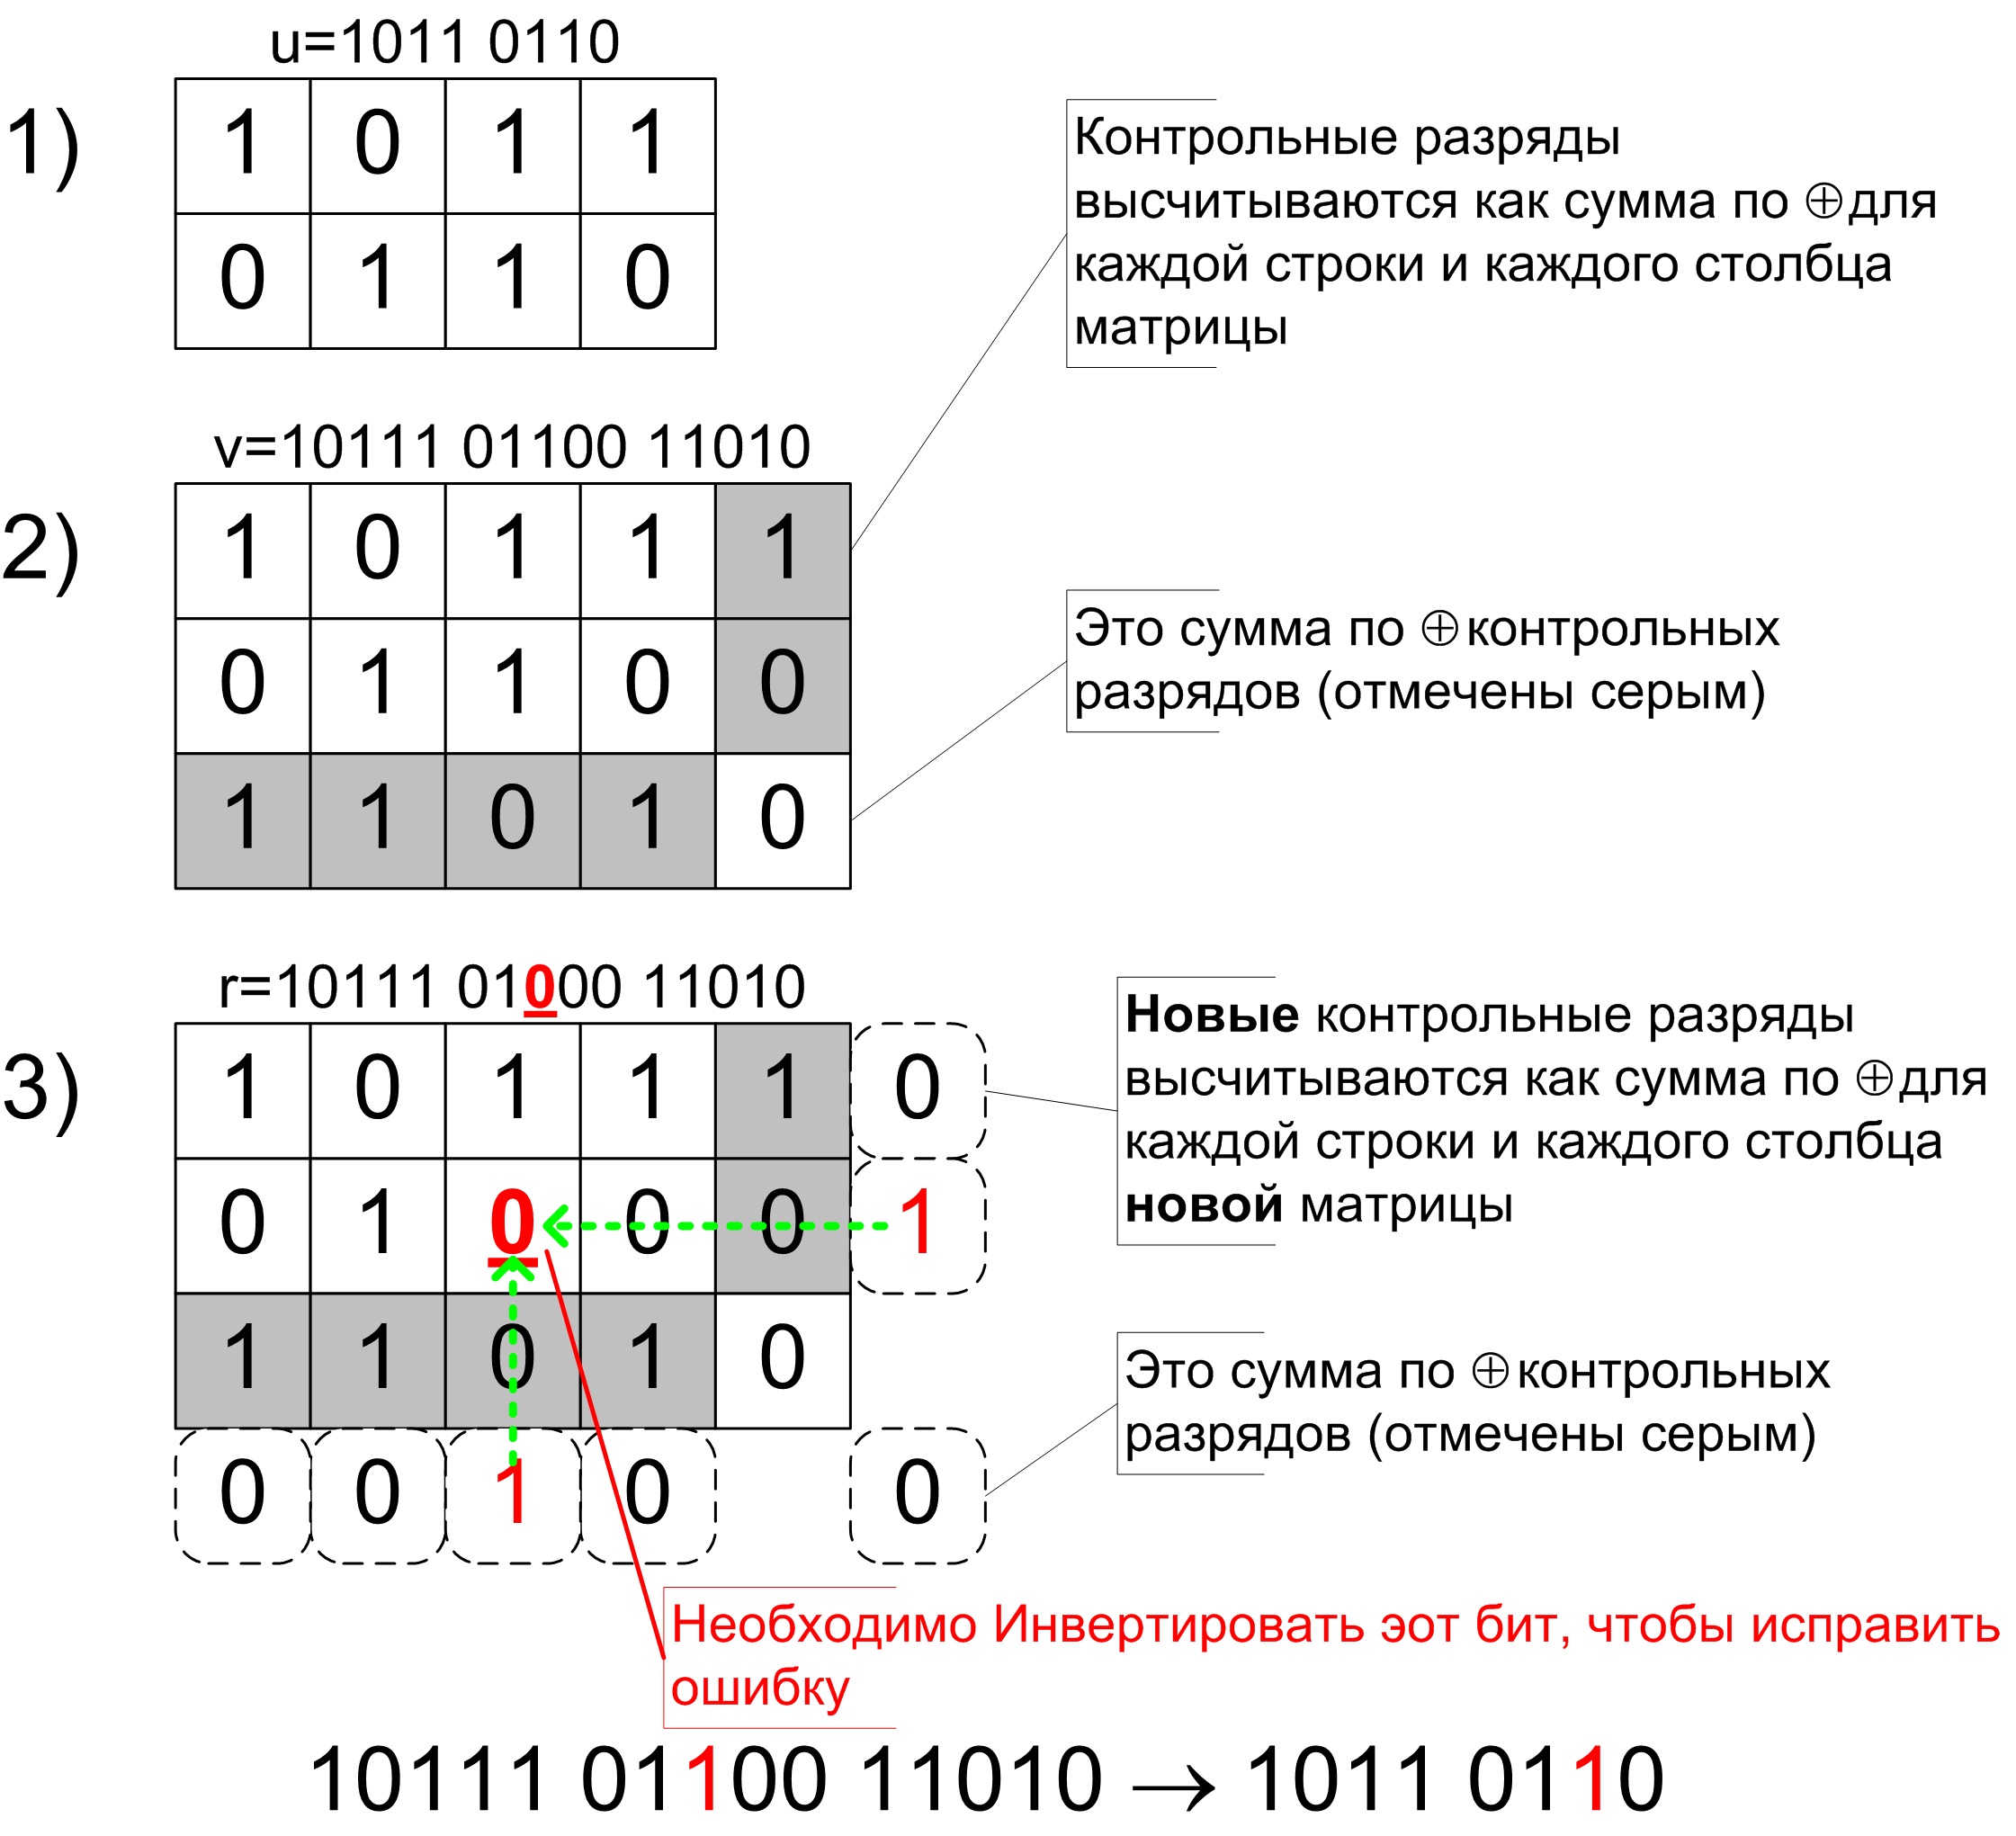
\includegraphics[width=.5\textwidth]{pict/matrix} } 
            \caption{Матричный контроль по четности}\label{pict:matrix}
        \end{center}
    \end{figure} 
    \mode<article>{См. Рис. \ref{pict:matrix}}
\end{frame}


Далее рассмотрим часто применяемый на практике код Хемминга, который дает максимальную экономию для FEC стратегии.

Рассмотрим, как сформировать код Хемминга в его классическом варианте. Код призван исправлять одиночные ошибки. Наиболее компактным будет код, который будет позволять находить номер разряда ошибочного бита. При этом пусть нулевой бит в таком представлении будет фиктивным и полученный от декодера нулевой номер ошибочного разряда будет означать, что ошибки не было. Таким образом, если необходимо передать исходное кодовое слово $u$ длиной $n$ бит, то нужно добавить к этому слову $m$ дополнительных (избыточных) бит исходя из равенства:
\[2^m\geq n+m+1.\]

\begin{frame}
    \frametitle{FEC}
    \framesubtitle{Классический код Хемминга. Кодирование}
    
    \[2^m\geq k+m+1, 2^{n-k}\geq n+1\] где $k$ --- длина информационного слова $u$; $m$ --- количество контрольных разрядов, $n=k+m$ --- длина получаемого кодового слова $v$.
    \begin{enumerate}
        \item В двоичном коде длиной $n=k+m$ бит контрольные $m$ бит следует разместить в разрядах с номерами, равными степени двойки ($2^0$,$2^1$,$2^2$,\ldots). Контрольные биты инициализируются нулём: $v_{2^i}=0$. $k$ бит информационного слова $u$ размещаются в оставшихся разрядах. Разряды нумеруются c $1$ справа-налево.
        
        \item \label{en:encode:recount} Каждый контрольный бит $v_{2^i}$ в разряде $2^i$ получается как сумма по модулю два бит кода, находящихся в разрядах, номера которых в двоичном представлении содержат $1$ в $i$-м разряде.
    \end{enumerate}
\end{frame}


\begin{frame}
    \frametitle{FEC}
    \framesubtitle{Классический код Хемминга. Декодирование}
    
    При декодировании контрольные разряды вектора $r$ пересчитываются как в п. \ref{en:encode:recount} на этапе кодирования. В результате в контрольных разрядах будет получено двоичное число --- номер разряда ошибочного бита в векторе $r$.
    \begin{example}
        Нужно передать $u=0011$ по каналу, в котором возможны одиночные ошибки.
    \end{example}
\end{frame}


\begin{frame}
    \frametitle{FEC}
    \framesubtitle{Классический код Хемминга. Пример кодирования}
    
    \begin{figure}
        \begin{center}
            \mode<presentation>{ 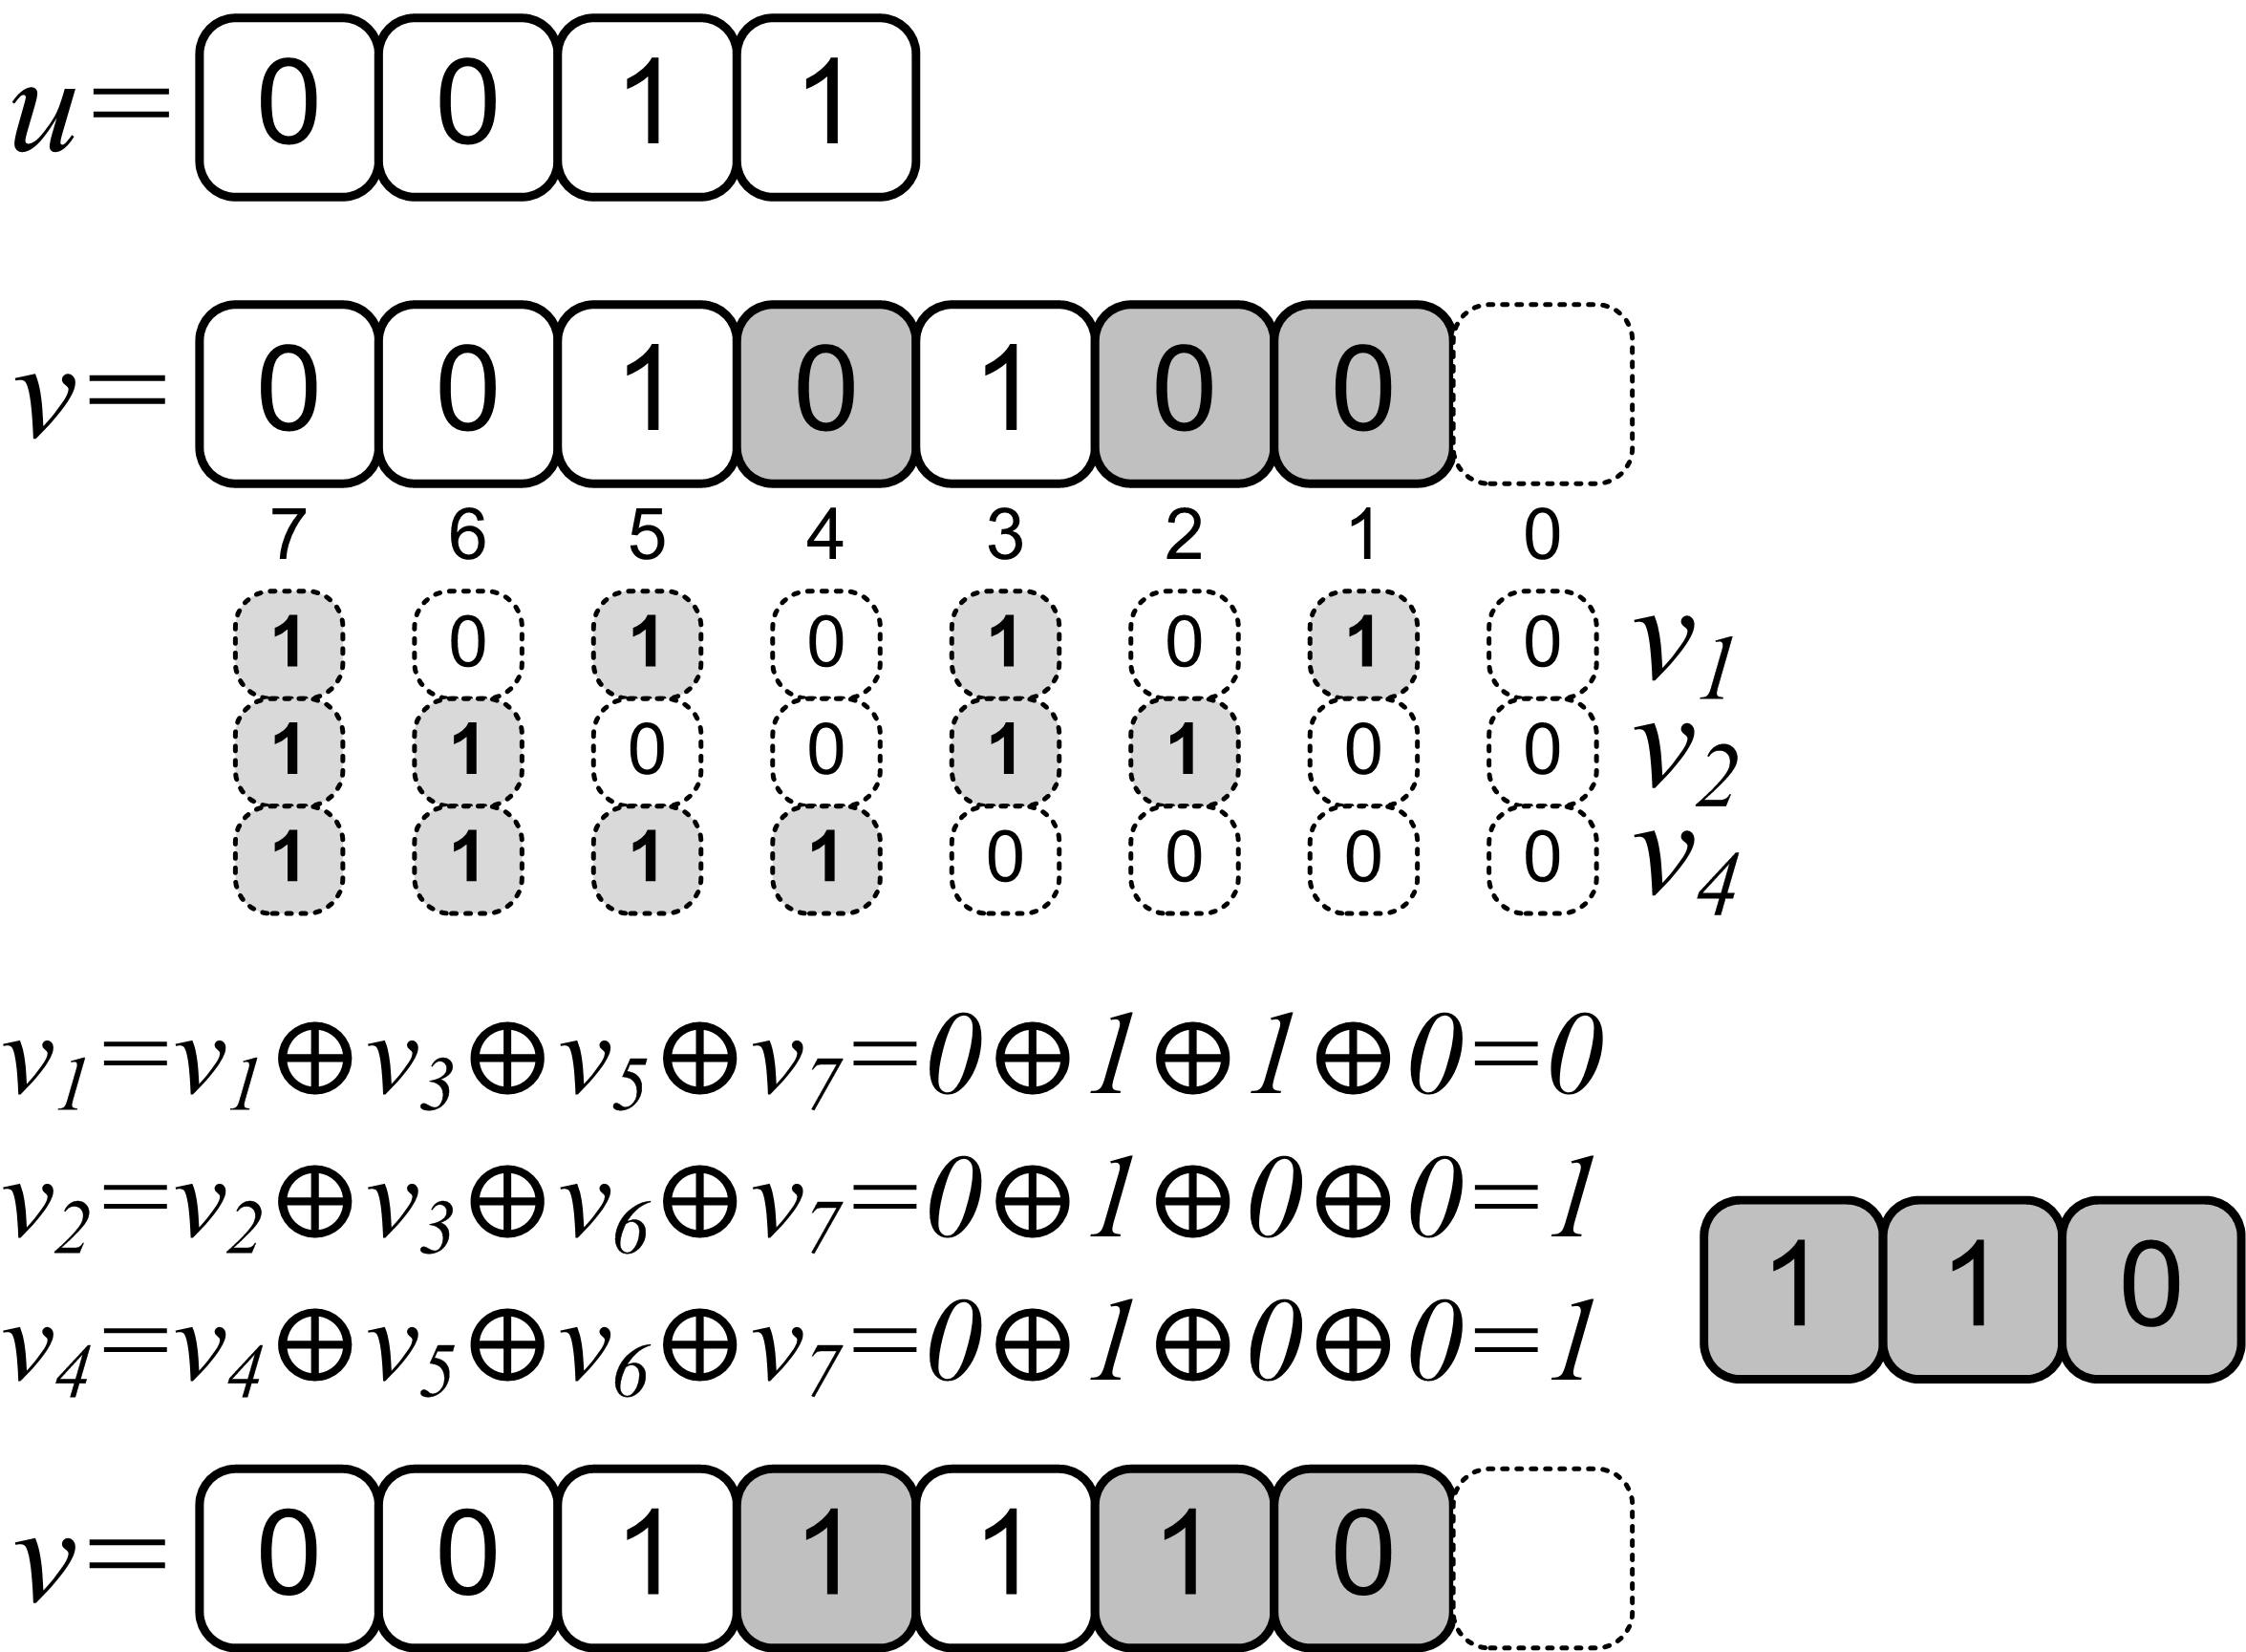
\includegraphics[height=.7\textheight]{pict/hammingEncode} }
            \mode<article>{ 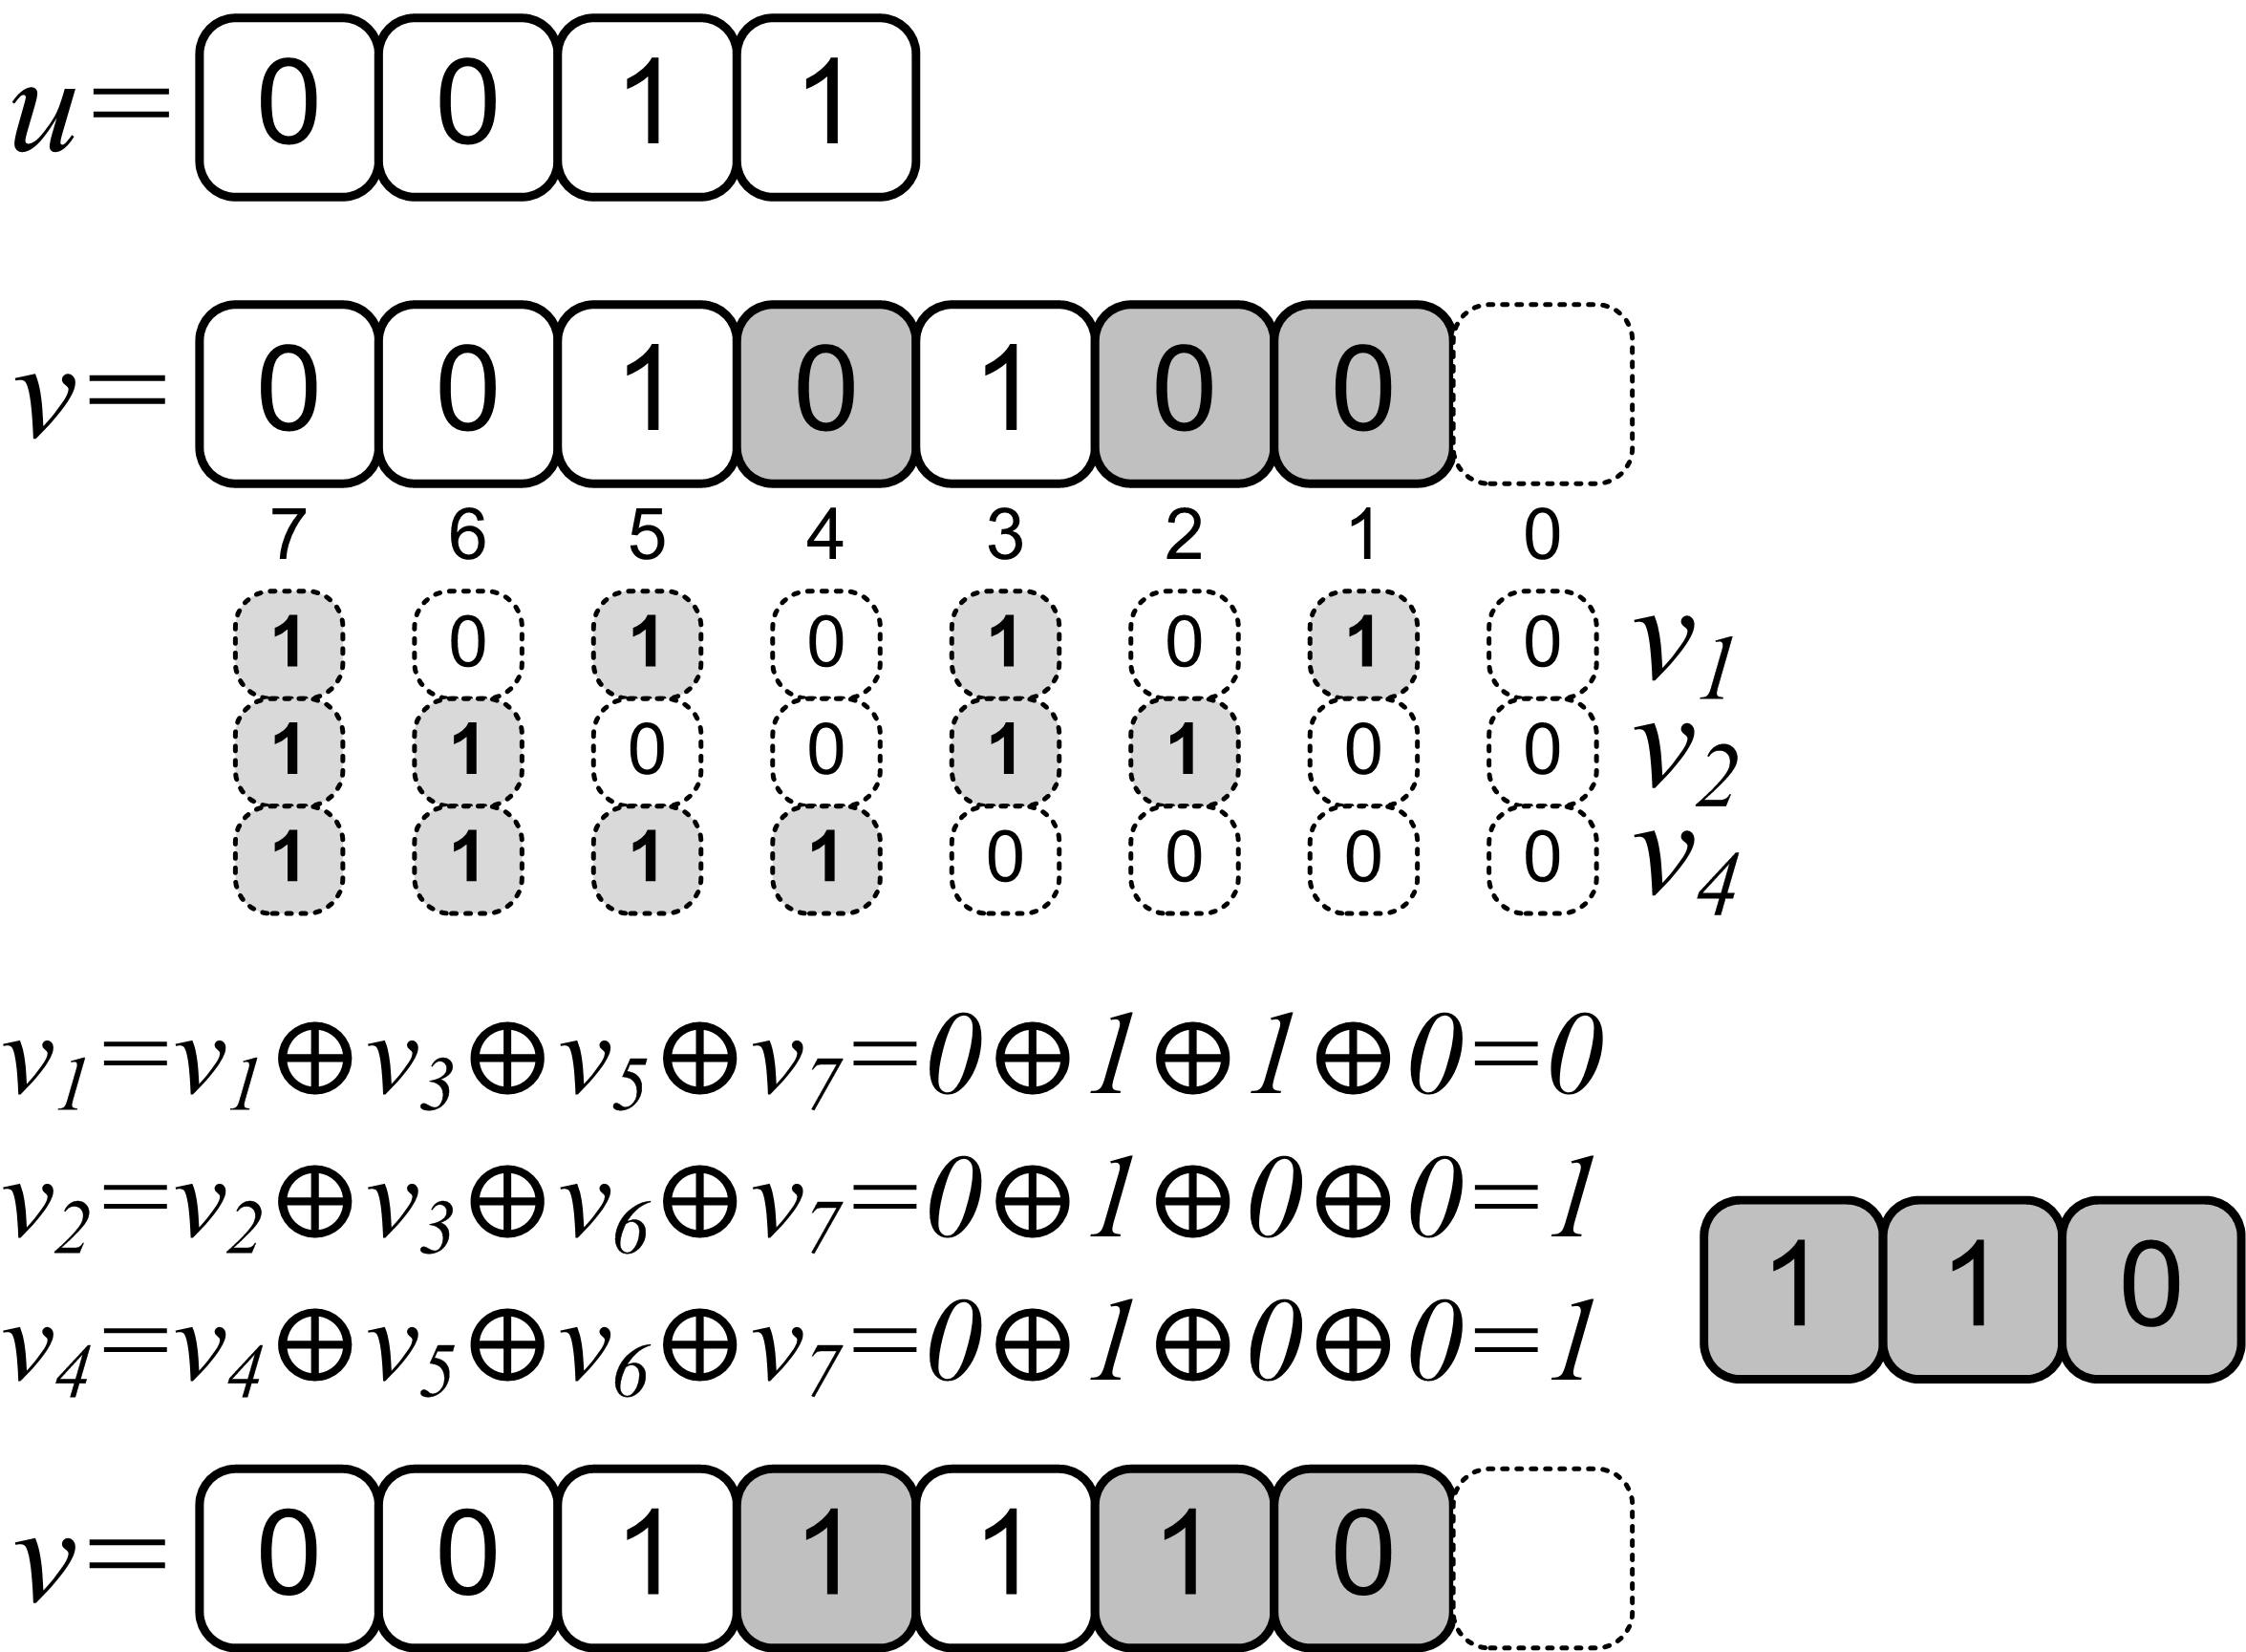
\includegraphics[width=.5\textwidth]{pict/hammingEncode} } 
            \caption{Код Хемминга. Пример кодирования}\label{pict:hammingEncode}
        \end{center}
    \end{figure}
    \mode<article>{См. Рис. \ref{pict:hammingEncode}}
\end{frame}


\begin{frame}
    \frametitle{FEC}
    \framesubtitle{Классический код Хемминга. Пример декодирования}
    
    \begin{figure}
        \begin{center}
            \mode<presentation>{ 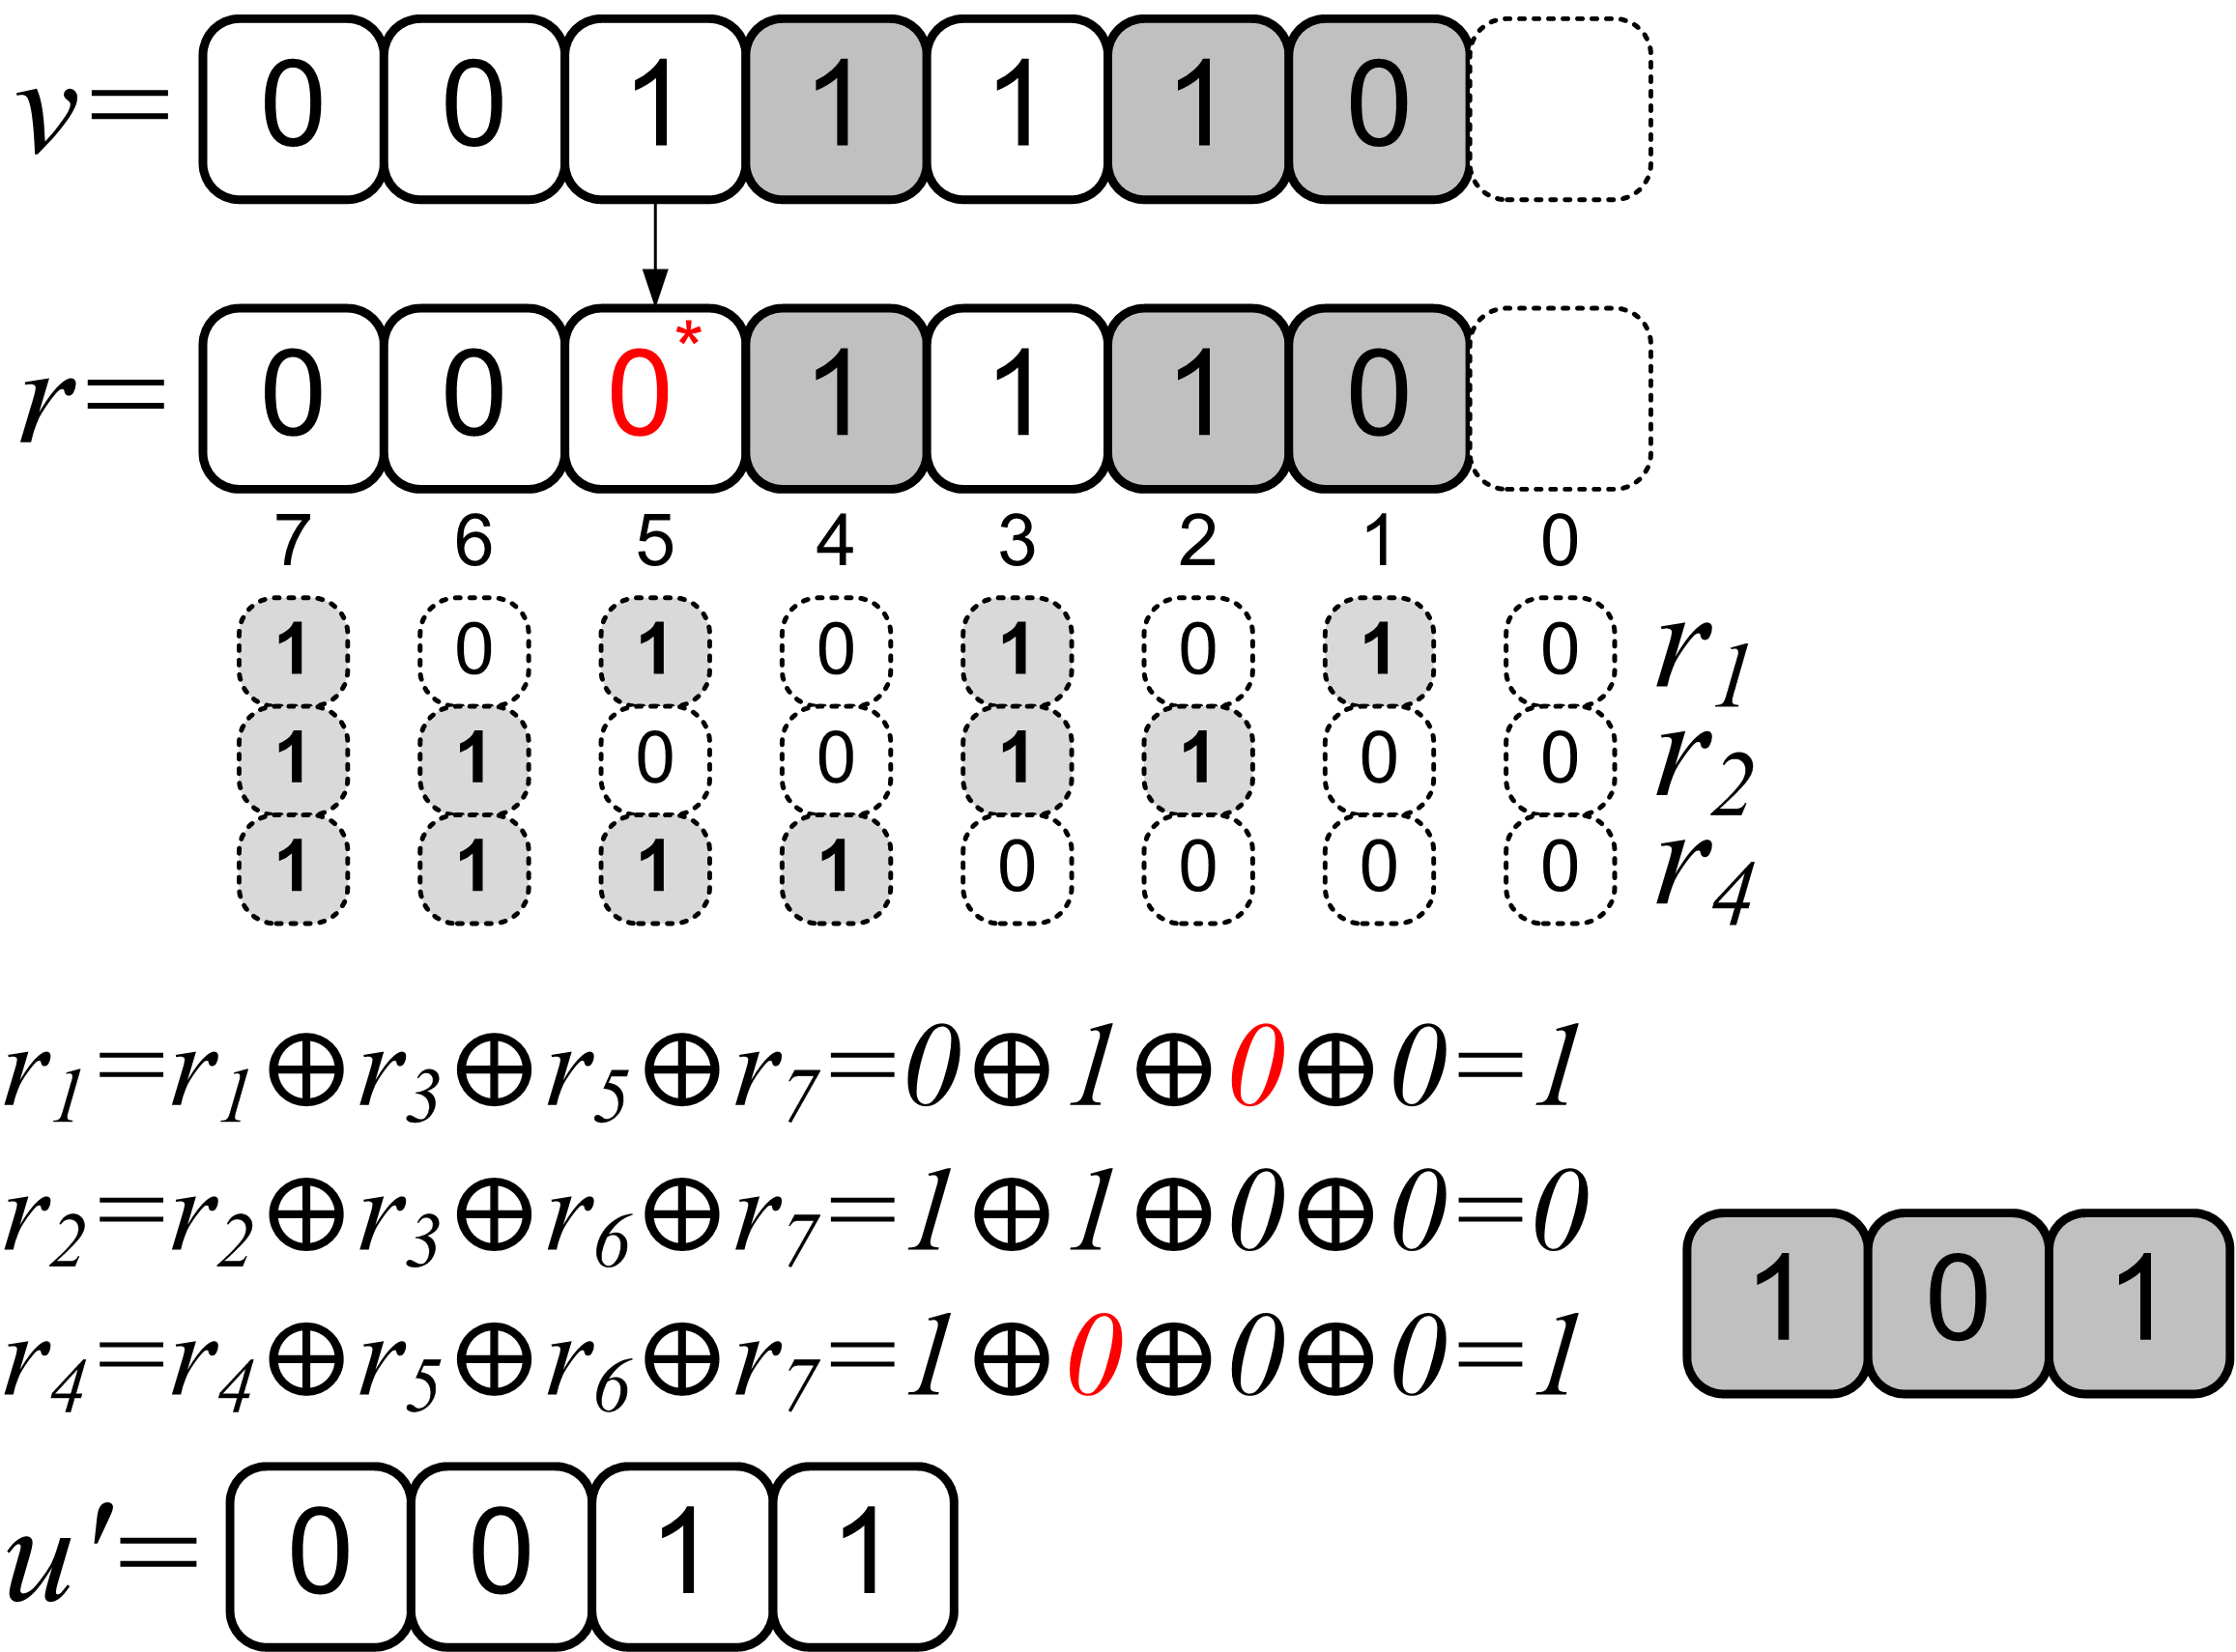
\includegraphics[height=.7\textheight]{pict/hammingDecode} }
            \mode<article>{ 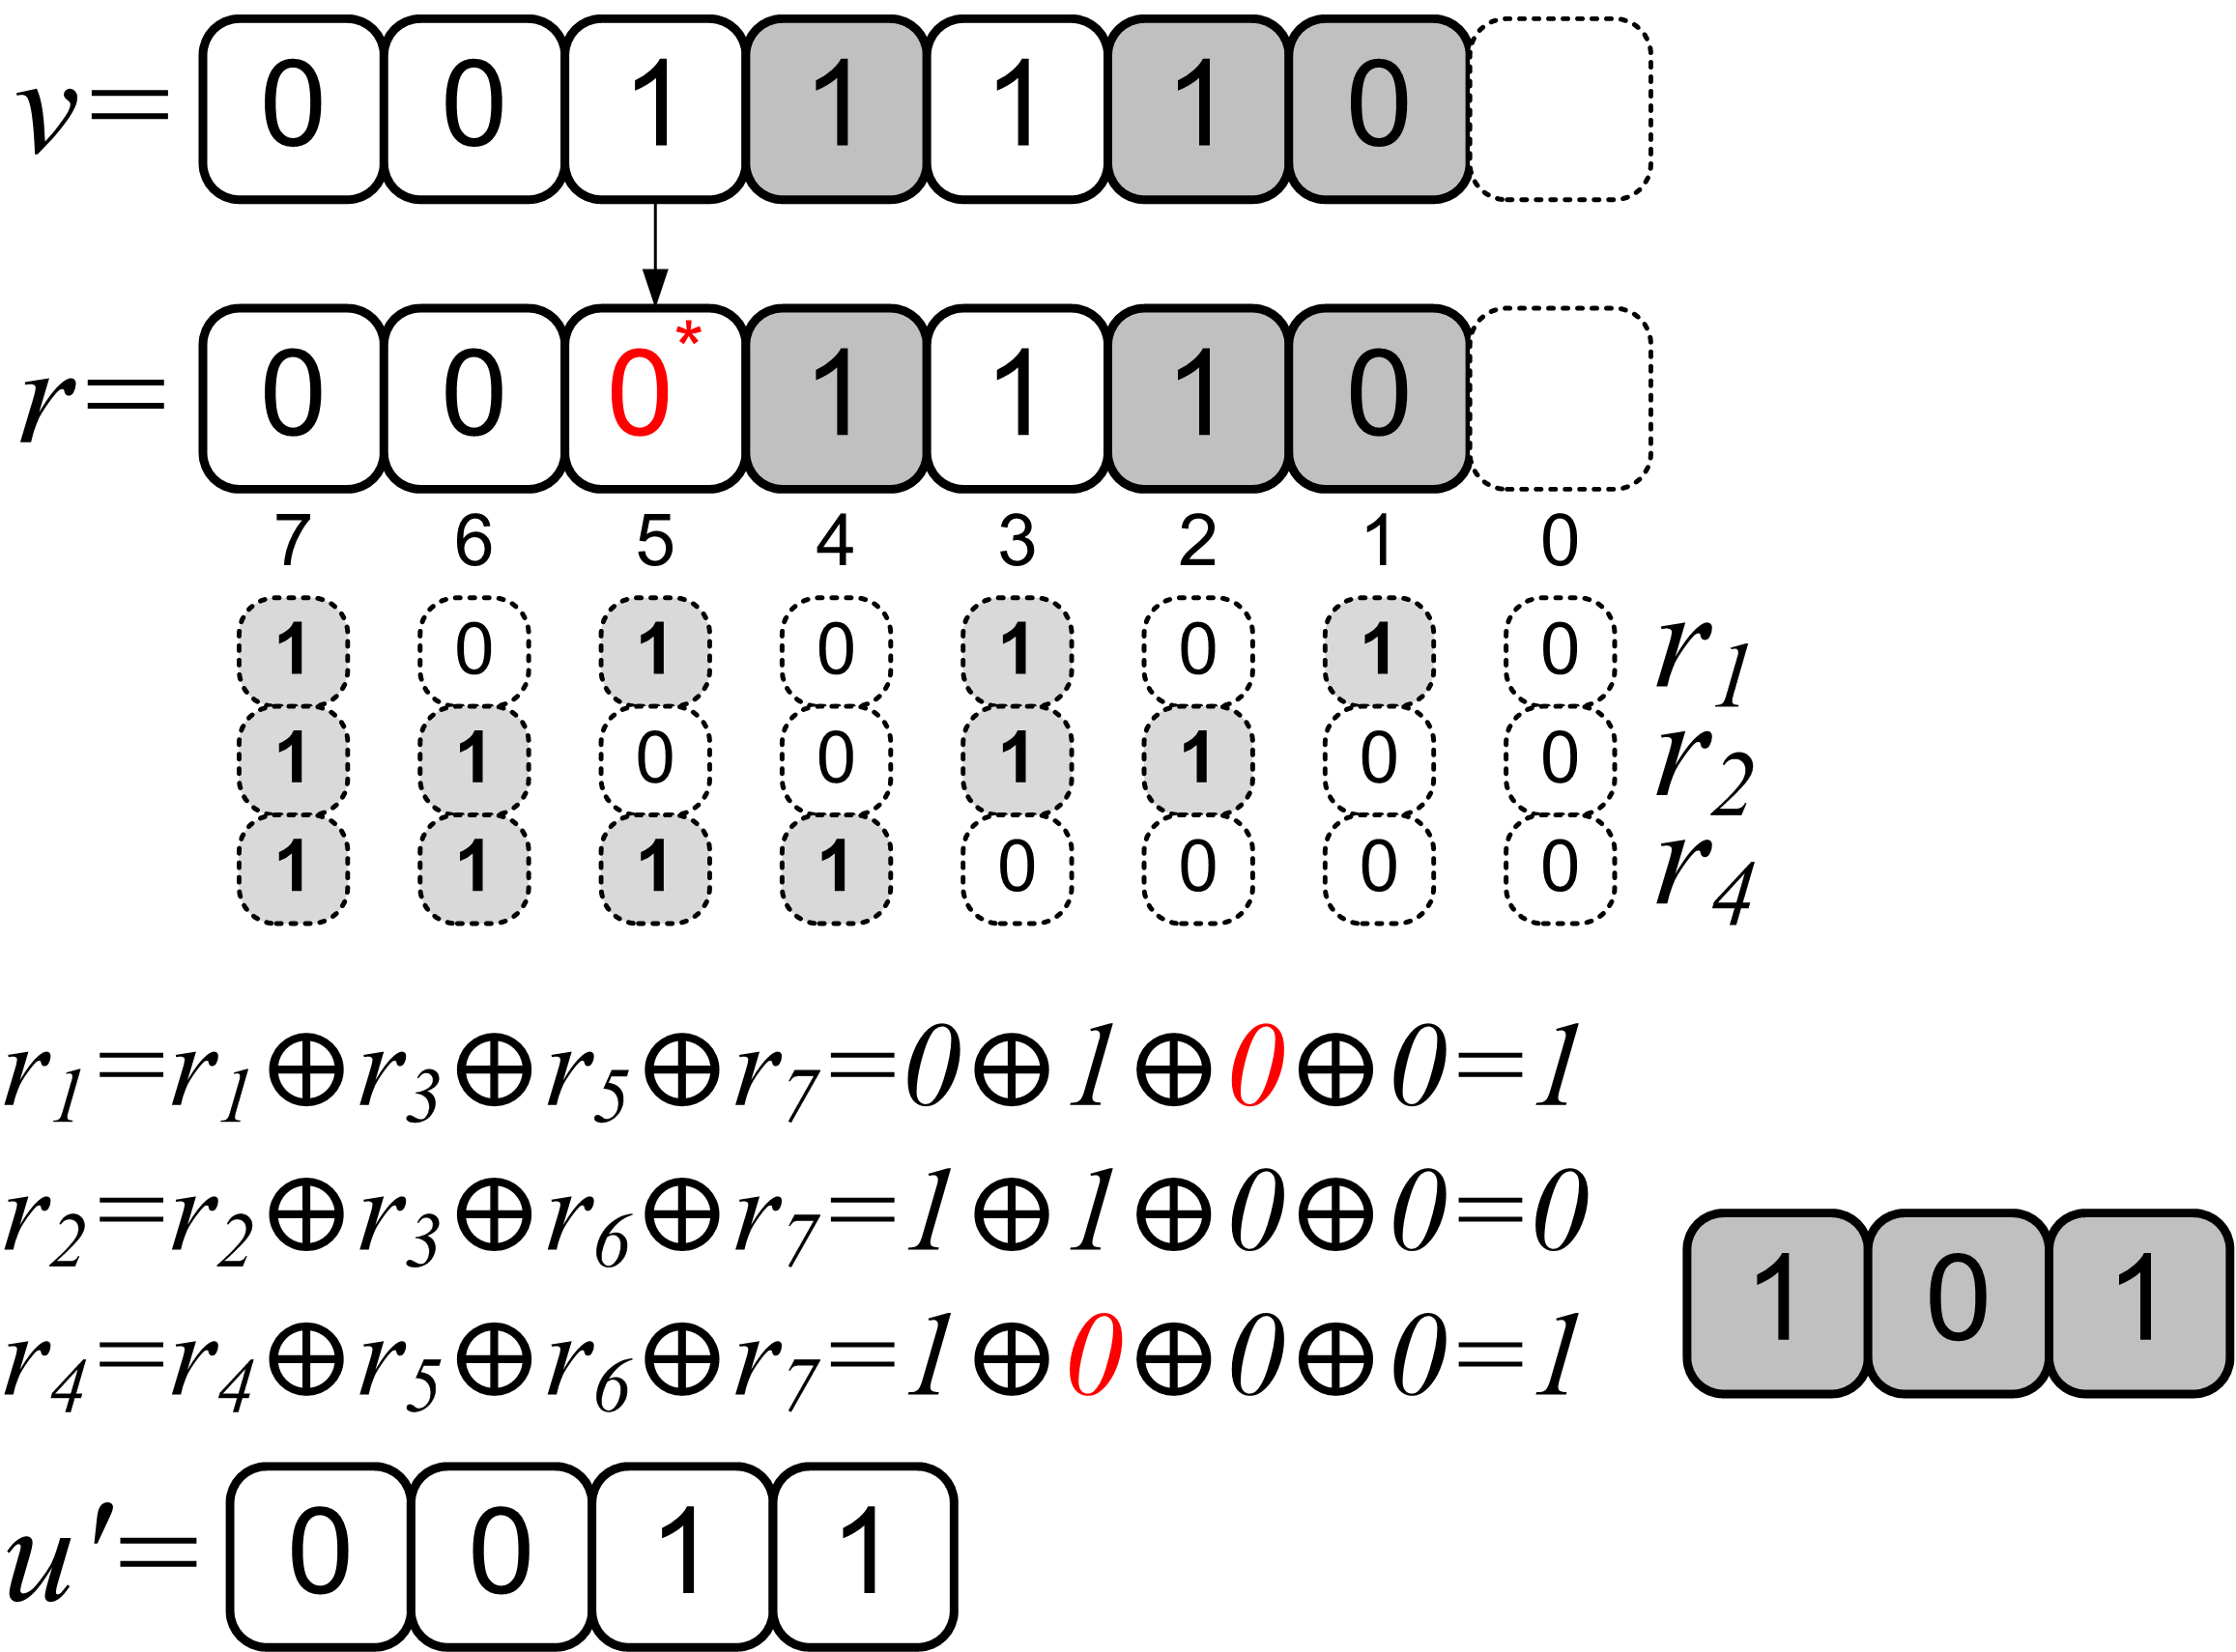
\includegraphics[width=.5\textwidth]{pict/hammingDecode} } 
            \caption{Код Хемминга. Пример исправления ошибки}\label{pict:hammingDecode}
        \end{center}
    \end{figure} 
    \mode<article>{См. Рис. \ref{pict:hammingDecode}}
\end{frame}


\appendix


\begin{frame}
    \frametitle{Источники}
    
    Предметное обсуждение помехоустойчивого кодирования можно найти в \cite{bib:verner:codingBase}.
    
    Математические основы помехоустойчивого кодирования изложены в \cite{bib:novic:discrmathprogrammer,bib:yablonsky:discreteintro}.
\end{frame}


\begin{frame}[allowframebreaks]{Библиография}
    \bibliographystyle{gost780u}
    \bibliography{./../bibliobase}
\end{frame}

\end{document}